%%%% ijcai20-multiauthor.tex

\typeout{IJCAI--PRICAI--20 Multiple authors example}

% These are the instructions for authors for IJCAI-20.

\documentclass{article}
\pdfpagewidth=8.5in
\pdfpageheight=11in
% The file ijcai20.sty is NOT the same than previous years'
\usepackage{ijcai20}

% Use the postscript times font!
\usepackage{times}
\renewcommand*\ttdefault{txtt}
\usepackage{soul}
\usepackage{url}
\usepackage[hidelinks]{hyperref}
\usepackage[utf8]{inputenc}
\usepackage[small]{caption}
\usepackage{graphicx}
\usepackage{amsmath}
\usepackage{booktabs}
\urlstyle{same}



\usepackage{setspace}
\usepackage{times}  %Required
\usepackage{helvet}  %Required
\usepackage{courier}  %Required
\usepackage{url}  %Required
%\usepackage{graphicx}  %Required

\usepackage{enumerate}


%\usepackage{algorithm}
%\usepackage{algorithmic}

\usepackage{amssymb}
\usepackage{enumerate}

\usepackage{subfigure}

\usepackage[linesnumbered,boxed,ruled,commentsnumbered]{algorithm2e}


% the following package is optional:
%\usepackage{latexsym}

% Following comment is from ijcai97-submit.tex:
% The preparation of these files was supported by Schlumberger Palo Alto
% Research, AT\&T Bell Laboratories, and Morgan Kaufmann Publishers.
% Shirley Jowell, of Morgan Kaufmann Publishers, and Peter F.
% Patel-Schneider, of AT\&T Bell Laboratories collaborated on their
% preparation.

% These instructions can be modified and used in other conferences as long
% as credit to the authors and supporting agencies is retained, this notice
% is not changed, and further modification or reuse is not restricted.
% Neither Shirley Jowell nor Peter F. Patel-Schneider can be listed as
% contacts for providing assistance without their prior permission.

% To use for other conferences, change references to files and the
% conference appropriate and use other authors, contacts, publishers, and
% organizations.
% Also change the deadline and address for returning papers and the length and
% page charge instructions.
% Put where the files are available in the appropriate places.

\title{On forgetting in CTL with Finite States: a preliminary report}

\author{
Renyan Feng$^1$\footnote{Contact Author}\and
Yisong Wang$^2$\and
Stefan Schlobach$^{3}$\And
Erman Acar$^4$\\
\affiliations
$^{1,2}$GuiZhou University\\
$^{3,4}$Vrije Universiteit Amsterdam\\
\emails
fengrenyan@gmail.com,
yswang@gzu.edu.cn,
\{k.s.schlobach, erman.acar\}@vu.nl
}

\begin{document}


\newcommand{\tuple}[1]{{\langle{#1}\rangle}}
\newcommand{\Mod}{\textit{Mod}}
\newcommand\ie{{\it i.e. }}
\newcommand\eg{{\it e.g.}}
%\newcommand\st{{\it s.t. }}
\newtheorem{definition}{Definition}
\newtheorem{examp}{Example}
\newenvironment{example}{\begin{examp}\rm}{\end{examp}}
\newtheorem{lemma}{Lemma}
\newtheorem{proposition}{Proposition}
\newtheorem{theorem}{Theorem}
\newtheorem{corollary}[theorem]{Corollary}
\newenvironment{proof}{{\bf Proof:}}{\hfill\rule{2mm}{2mm}\\ }
\newcommand{\rto}{\rightarrow}
\newcommand{\lto}{\leftarrow}
\newcommand{\lrto}{\leftrightarrow}
\newcommand{\Rto}{\Rightarrow}
\newcommand{\Lto}{\Leftarrow}
\newcommand{\LRto}{\Leftrightarrow}
\newcommand{\Var}{\textit{Var}}
\newcommand{\Forget}{\textit{Forget}}
\newcommand{\KForget}{\textit{KForget}}
\newcommand{\TForget}{\textit{TForget}}
%\newcommand{\forget}{\textit{forget}}
\newcommand{\Fst}{\textit{Fst}}
\newcommand{\dep}{\textit{dep}}
\newcommand{\term}{\textit{term}}
\newcommand{\literal}{\textit{literal}}

\newcommand{\Atom}{\mathcal{A}}
\newcommand{\SFive}{\textbf{S5}}
\newcommand{\MPK}{\textsc{k}}
\newcommand{\MPB}{\textsc{b}}
\newcommand{\MPT}{\textsc{t}}
\newcommand{\MPA}{\forall}
\newcommand{\MPE}{\exists}

\newcommand{\DNF}{\textit{DNF}}
\newcommand{\CNF}{\textit{CNF}}

\newcommand{\degree}{\textit{degree}}
\newcommand{\sunfold}{\textit{sunfold}}

\newcommand{\Pos}{\textit{Pos}}
\newcommand{\Neg}{\textit{Neg}}
\newcommand\wrt{{\it w.r.t.}}
\newcommand{\Hm} {{\cal M}}
\newcommand{\Hw} {{\cal W}}
\newcommand{\Hr} {{\cal R}}
\newcommand{\Hb} {{\cal B}}
\newcommand{\Ha} {{\cal A}}

\newcommand{\Dsj}{\triangledown}

\newcommand{\wnext}{\widetilde{\bigcirc}}
\newcommand{\nex}{\bigcirc}
\newcommand{\ness}{\square}
\newcommand{\qness}{\boxminus}
\newcommand{\wqnext}{\widetilde{\circleddash}}
\newcommand{\qnext}{\circleddash}
\newcommand{\may}{\lozenge}
\newcommand{\qmay}{\blacklozenge}
\newcommand{\unt} {{\cal U}}
\newcommand{\since} {{\cal S}}
\newcommand{\SNF} {\textit{SNF$_C$}}
\newcommand{\start}{\textbf{start}}
\newcommand{\Elm}{\textit{Elm}}
\newcommand{\simp}{\textbf{simp}}
\newcommand{\nnf}{\textbf{nnf}}

\newcommand{\CTL}{\textrm{CTL}}
\newcommand{\Ind}{\textrm{Ind}}
\newcommand{\Tran}{\textrm{Tran}}
\newcommand{\Sub}{\textrm{Sub}}
\newcommand{\forget}{{\textsc{f}_\CTL}}
\newcommand{\ALL}{\textsc{a}}
\newcommand{\EXIST}{\textsc{e}}
\newcommand{\NEXT}{\textsc{x}}
\newcommand{\FUTURE}{\textsc{f}}
\newcommand{\UNTIL}{\textsc{u}}
\newcommand{\GLOBAL}{\textsc{g}}
\newcommand{\UNLESS}{\textsc{w}}
\newcommand{\Def}{\textrm{def}}
\newcommand{\IR}{\textrm{IR}}
\newcommand{\Tr}{\textrm{Tr}}
\newcommand{\dis}{\textrm{dis}}
\def\PP{\ensuremath{\textbf{PP}}}
\def\NgP{\ensuremath{\textbf{NP}}}
\def\W{\ensuremath{\textbf{W}}}
\newcommand{\Pre}{\textrm{Pre}}
\newcommand{\Post}{\textrm{Post}}


\newcommand{\CTLsnf}{{\textsc{SNF}_{\textsc{ctl}}^g}}
\newcommand{\ResC}{{\textsc{R}_{\textsc{ctl}}^{\succ, S}}}
\newcommand{\CTLforget}{{\textsc{F}_{\textsc{ctl}}}}
\newcommand{\Refine}{\textsc{Refine}}
\newcommand{\cf}{\textrm{cf.}}
\newcommand{\NEXP}{\textmd{\rm NEXP}}
\newcommand{\EXP}{\textmd{\rm EXP}}
\newcommand{\coNEXP}{\textmd{\rm co-NEXP}}
\newcommand{\NP}{\textmd{\rm NP}}
\newcommand{\coNP}{\textmd{\rm co-NP}}
\newcommand{\Pol}{\textmd{\rm P}}
\newcommand{\BH}[1]{\textmd{\rm BH}_{#1}}
\newcommand{\coBH}[1]{\textmd{\rm co-BH}_{#1}}
\newcommand{\Empty}{\varnothing}
\newcommand{\NLOG}{\textmd{\rm NLOG}}
\newcommand{\DeltaP}[1]{\Delta_{#1}^{p}}
\newcommand{\PIP}[1]{\Pi_{#1}^{p}}
\newcommand{\SigmaP}[1]{\Sigma_{#1}^{p}}



\maketitle

\begin{abstract}
Computation Tree Logic (\CTL) is one of the main logical formalisms for program specification, which prescribes what a transition system has to do and what not, and verification.
How to extract relevant specification from existing specification is a key problem when facing a big database of specification.
Forgetting, as a technology distilling from a knowledge base only the part that is relevant to a subset of alphabet, just happens to solve the problem talked above.
In this paper, we study forgetting in \CTL\ from the sematic forgetting point of view by bisimulation to distill from a set of specifications only the part that is relevant to a subset of the alphabet.
And we show that the \CTL\ system is closed under forgetting.
Besides, from the point of view of model and resolution, this paper discusses the algorithms of computing forgetting on \CTL.

%Keywords: Forgetting, \CTL, Bisimulation, Specification, Resolution.
\end{abstract}

\section{Introduction}

 \emph{Temporal logic} has found numerous applications in computer science, ranging from the traditional and well-developed fields of program specification and verification~\cite{manna1995temporal,pnueli1992temporal,pnueli1986applications}, temporal databases~\cite{chomicki1994temporal,chomicki1995feasibility,abiteboul1996temporal,sernadas1980temporal}, and distributed and multi-agent systems~\cite{fagin2004reasoning}, to more recent uses in knowledge representation and reasoning~\cite{schild1993combining,baader1995multi,hodkinson2000decidable}. In temporal logic model checking, a kind of verification, temporal logic is mainly to use describe the properties of the system. Two important families of temporal logics have been considered: linear-time temporal logics (e.g LTL\cite{pnueli1977temporal}) can be used to express properties of one single execution of the system under study, while branching-time temporal logics(e.g CTL\cite{clarke1981design} and CTL*~\cite{emerson1986sometimes})consider the execution tree~\cite{laroussinie2014quantified}. In this paper, we are interested to branching-time temporal logic-CTL (Computation Tree temporal Logic).

 A \emph{specification} often refers to a set of documented requirements to be satisfied by a material, design, product, or service ?1?. In model checking, specification is mainly used to specify the properties that should be satisfied by system~\cite{chaki2005concurrent,chaki2004expressive,clarke1994model,ghosh2016arsenal}. The practical effectiveness of model checking is characterized by a trade-off between the expressive power of the specification formalism and the complexity of the corresponding model checking algorithm~\cite{chaki2004expressive}. For software verification, this problem is even more acute, since software is harder to specify, and state explosion is exacerbated by the concurrent execution of multiple components. In order to solve the problem of states exploring, in the last few decades, researchers have put forward Modular Verification, rather than consider the whole states space~\cite{chaki2005concurrent,chaki2004expressive}. However, the elements in a module is almost different with the other modules. If we can extract those knowledge related to the elements in this module, then it can be more efficient to verification. In addition, as the system has been updated, some of the elements previously considered are no longer considered, if we have had those specifications, we do not need to reproduce the specifications that different with the original one only in that the latter using lesser atoms. Besides, with the size of the system growing, not only has the number of available (proposition) increased considerably, but they are often large in size and are becoming more complex to manage. This leads to the specification being difficult to maintain and modify, and costly to reuse for later processing, where only a specific part of an specification is of interest. All of this working directly on the whole of the original specification and building a new sub-specification are unadvisable. Therefore, a strong demand for techniques and automated tools for obtaining the specific sub-specification.

 \emph{Forgetting}, as a technology distilling from a knowledge base only the part that is relevant to a subset of alphabet, just happens to solve the problem talked above.
 For example, the is a theory $T=\{a \vee \neg b, c \wedge b\}$ in Classical Proposition Logic (CPL), a theory that the $\{a, c\}$-alphabet related part of $T$ is $\{a\vee c\}$.
  Although there have been a number of studies on similar methods of forgetting, such as variable elimination, irrelevance and independence\cite{bobrow1997special}, forgetting has been put forward by Lin at first~\cite{lin1994forget}. Over the last twenty years, researchers have developed forgetting notions and theories not only in classical logic but also in other non-classical logic systems, such as forgetting in logic programs under answer set/stable model semantics~\cite{DBLP:Zhang:AIJ2006,Eiter2008Semantic,Wong:PhD:Thesis,Yisong:KR:2012,Yisong:IJCAI:2013}, forgetting in description logic~\cite{Wang:AMAI:2010,Lutz:IJCAI:2011,zhao2017role} and knowledge forgetting in modal logic~\cite{Zhang2009Knowledge,Kaile:JAIR:2009,Yongmei:IJCAI:2011,fang2019forgetting}. In application, forgetting has been used in planning~\cite{lin2003compiling},  conflict solving \cite{Lang2010Reasoning,Zhang2005Solving}, knowledge compilation \cite{Zhang2009Knowledge,Bienvenu2010Knowledge}, createing restricted views of ontologies~\cite{ZhaoSchmidt18a}, strongest and weakest definitions \cite{Lang2008On}, strongest necessary and weakest
sufficient conditions \cite{lin2001strongest} and so on. Besides, (semantic) forgetting is studied by researchers in \cite{Marquis2003Propositional,Eiter2008Semantic}.  To our best knowledge, though forgetting has been extensively investigated from various aspects of different logical systems, in standard propositional logic, a general algorithm of forgetting and its computation-oriented investigation in CTL are still lacking.
However, as we said above that this skill is essential in CTL. A simple example in the follows show the necessity of forgetting in CTL:
\begin{itemize}
  \item \emph{Let $\varphi = \ALL((p\wedge q) \UNTIL (f\vee m))\wedge r$, then what is the $\{q,f,m,r\}$-alphabet related part of $\varphi$?}
\end{itemize}
Apparent that this is not easy to obtain even for this simple $\varphi$. More critical is existing methods cannot solve the problem.
In this paper we will introduce a skill that can solve this problem.

It is know that forgetting can be defined in two closely related ways: it can be defined on
the syntactic level as the dual of uniform interpolation~\cite{konev2009forgetting} and it can be defined model-theoretically as semantic forgetting~\cite{zhao2017role}.
Besides, forgetting, is regarded as an abstract belief change operator, independent of
the underlying logic, is reached by James P.~\cite{DBLP:journals/jair/Delgrande17}.
In this paper, we explore the forgetting in CTL from a semantic forgetting point of view. Bisimulation, a concept weaker than homogeneous and stronger than homomorphic, make it possible to relate systems described at different levels of abstraction and to verify, for example, the correctness of an implementation with respect to a more abstract specification of a given system~\cite{DBLP:reference/mc/ClarkeHV18}. Bisimulation was first proposed by Benthem~\cite{Benthem1977Modal}, and
then have been used in analyzing the expressive power of modal logics and in Model checking~\cite{Baier:PMC:2008}. The difference between our concept and these concepts include two aspects. On one hand, we have introduced the set $V$ of atoms, which dose not mentioned in transition system. On the other hand, our $V$-bisimulation is on the set of Kripke structures, not on the set of states as before. Through this generalization, we were able to compare the differences among the Kripke structures on the set $V$, which allowed us to explore semantically the meaning of forgetting the atomic set $V$ in the CTL.



The forgetting is close in the classical propositional logic (CPL), that is the result of forgetting a set $V$ of atoms from the CPL formula is also a CPL formula. However, there are some logic systems, such as first-order logic and descrp logic, the forgetting is not close. Fortunately, our concept of forgetting is closed in the CTL and in order to prove this result, we introduced the characteristic formula. As its name suggests, the characteristic formula is a formula that describes a Kripke structure. I It describes the structure that the Kripke structure has and the meaning it conveys. The characteristic formula in CTL was originally proposed by~\cite{DBLP:journals/tcs/BrowneCG88}. In this paper, it is modified on the original basis and combined with our v-bisimulation semantics. We don't care about the characteristic formula of the Kripke structure in the whole proposition space. We only consider its characteristic formula on a specified set.


\textbf{Our\ Contributions:} Focusing on forgetting in CTL, this article has the following contributions:
\begin{itemize}
  \item Proposed a new set-based bisimulation for transition system;
  \item Given the definition of forgetting in CTL;
  \item Defined the characteristic formula of a Kripke structure on some set $V$ of atoms;
  \item Proved that the forgetting in CTL is closed;
  \item Two algorithms have been proposed for computing forgetting in CTL.
\end{itemize}

The rest of the paper is organised as follows. Section 2 introduces the related notions for forgetting in \CTL, including the syntax and semantics of \CTL, the language we aimed for, and it's normal form.
A formal definition of concept forgetting for \CTL\ follows in Section 3.
From the point of view of model and resolution, we propose two algorithms of computing forgetting on \CTL\ in Section 4.
%In Section 5, we propose an algorithm to judge whether two structures are $V$-bisimular.
% Section 6 explores the relation between forgetting and SNC (WSC) that is the application of forgetting in SNC (WSC).
 We conclude in Section 5 with a summary of the work and an outline of directions of future work.
 Besides, in the appendix we give the proofs of main results in this paper.

 \section{Preliminaries}
We start with some technical and notational preliminaries. Throughout this paper, we fix a finite set $\Ha$ of propositional variables (or atoms), and use $V$, $V'$ for subsets of $\Ha$. In the following several parts, we will introduce the structure we use for \CTL, syntactic and semantic of \CTL\ and the normal form $\CTLsnf$ (Separated Normal Form with Global Clauses for \CTL) of \CTL~\cite{zhang2009refined}.
\subsection{Model structure in \CTL}
 In general, a transition system~\footnote{According to \cite{Baier:PMC:2008},
a {\em transition system} TS is a tuple $(S, Act,\rto,I, AP, L)$ where
(1) $S$ is a set of states,
(2) $\textrm{Act}$ is a set of actions,
(3) $\rto\subseteq S\times \textrm{Act}\times S$ is a transition relation,
(4) $I\subseteq S$ is a set of initial states,
(5) $\textrm{AP}$ is a set of atomic propositions, and
(6) $L:S\rto 2^{\textrm{AP}}$ is a labeling function.} is described as a \emph{model\ structure} (or \emph{Kripke \ structure})(in this article, we treat transition system and model structure as the same thing), and a model structure is a triple $\Hm=(S,R,L)$~\cite{emerson1990temporal}, where
\begin{itemize}
  \item $S$ is a set of states,
  \item $R\subseteq S\times S$ is a total binary relation over $S$, \ie, for each state $s\in S$ there is a state $s'\in S$ such that $(s,s')\in R$, and
  \item $L$ is an interpretation function $S\rto 2^{\cal A}$ mapping every state to the set of atoms true at that state.
\end{itemize}
In this article, the same as~\cite{DBLP:journals/tcs/BrowneCG88}, all of our results apply only to finite Kripke structures.
Besides, we restrict ourselves to model structure $\Hm=(S,R,L,s_0)$ (similar with that in~\cite{zhang2009refined}) such that
\begin{itemize}
  \item there exists a state $s_0$, called the \emph{initial\ state}, such that for every state $s\in S$ there is a path $\pi_{s_0}$ s.t. $s\in \pi_{s_0}$.
\end{itemize}
We call a model structure $\Hm$ on a set $V$ of atoms if $L: S \rto 2^V$, \ie, the labeling function $L$ map every state to $V$ (not the $\Ha$).  A \emph{path} $\pi_{s_i}$ start from $s_i$ of $\Hm$ is a infinite sequence of states $\pi_{s_i}=(s_i, s_{i+1} s_{i+2},\dots)$, where for each $j$ ($i\leq j$), $(s_j, s_{j+1}) \in R$. By $s'\in \pi_{s_i}$ we mean that $s'$ is a state in the path $\pi_{s_i}$.

For a given model structure $(S,R,L,s_0)$ and $s\in S$,
the {\em computation tree}
$\Tr_n^{\cal M}(s)$ of $\cal M$(or simply $\Tr_n(s)$), that has depth $n$ and is rooted at $s$, is recursively defined as~\cite{DBLP:journals/tcs/BrowneCG88}, for $n\ge 0$,
\begin{itemize}
  \item $\Tr_0(s)$ consists of a single node $s$ with label $s$.
  \item $\Tr_{n+1}(s)$ has as its root a node $m$ with label  $s$, and
  if $(s,s')\in R$ then the node $m$ has a subtree $\Tr_n(s')$\footnote{Though
  some nodes of the tree may have the same label, they are different nodes in the tree.}.
\end{itemize}
By $s_n$ we mean the node at the $n$th level in tree $\Tr_m(s)$ $(m \geq n)$.

A {\em \MPK-structure} (or {\em \MPK-interpretation}) is a model structure
${\cal M}=(S, R, L, s_0)$ associating
with a state $s\in S$, which is written as $({\cal M},s)$ for convenience in the following.
In the case $s$ is an initial state of $\cal M$, the \MPK-structure is {\em initial}.


\subsection{Syntactic and semantic of \CTL}
In the following we briefly review the basic syntax and semantics
of the {\em Computation Tree Logic}
(\CTL\ in short)~\cite{DBLP:journals/toplas/ClarkeES86}. %Huth:BOOK:1999}.
%In  $\cal L$, the model of time is a tree-like structure in which the future is not
%determined; there are different paths in the future, any one of which might
%be the `actual' path that is realized.
%
The {\em signature} of $\cal L$ includes:
\begin{itemize}
  \item a finite set of Boolean variables, called {\em atoms} of $\cal L$: $\cal A$;
  \item the classical connectives: $\bot,\lor$ and $\neg$;
  \item the path quantifiers: $\ALL$ and $\EXIST$;
  \item the temporal operators: \NEXT, \FUTURE, \GLOBAL\, \UNTIL\ and \UNLESS, that
  means `neXt state', `some Future state', `all future states (Globally)', `Until' and `Unless', respectively;
  \item parentheses: ( and ).
\end{itemize}

The {\em (existential normal form or ENF in short) formulas} of
$\cal L$ are inductively defined via a Backus Naur form:
\begin{equation}\label{def:CTL:formulas}
  \phi ::= \bot\mid p \mid\neg\phi \mid \phi\lor\phi \mid
    \EXIST \NEXT \phi \mid
    %\EXIST \FUTURE \phi \mid
    \EXIST \GLOBAL \phi \mid
    \EXIST [\phi\ \UNTIL\ \phi]%.% \mid
    %\ALL \NEXT \phi \mid
%    \ALL \FUTURE \phi \mid
%    \ALL \GLOBAL \phi \mid
%    \ALL [\phi\ \UNTIL\ \phi]
\end{equation}
where $p\in\cal A$. The formulas $\phi\land\psi$ and $\phi\rto\psi$
are defined in a standard manner of propositional logic. Intuitively,
the formula $\EXIST\NEXT\phi$ means that $\phi$ holds in some immediate successor
of the current program state; the formula $\EXIST\GLOBAL\phi$ means
that for some computation path $\phi$ holds at every state along the path; and the
formula $\EXIST[\phi\UNTIL\psi]$ means that
for some computation path there is an initial prefix of the path such
that $\psi$ holds at the last state of the prefix  and $\phi$ holds at all other
states along the prefix.
The other form formulas of $\cal L$ are abbreviated as follows
using the forms of (\ref{def:CTL:formulas}):
\begin{align*}
  & \top =_{\Def} \neg\bot,\\
  & \ALL [\phi\ \UNTIL\ \psi] =_{\Def}
    \neg(\EXIST[\neg\psi\UNTIL \left(\neg \phi\land\neg\psi)]\lor\EXIST\GLOBAL\neg\psi\right),\\
  & \ALL\FUTURE\phi=_{\Def}   \ALL [\top \UNTIL\ \phi],\\
  & \EXIST\FUTURE\phi=_{\Def}\EXIST[\top\UNTIL\phi],\\
  & \ALL\GLOBAL\phi =_{\Def} \neg\EXIST\FUTURE\neg\phi,\\
  & \ALL\NEXT\phi =_{\Def} \neg\EXIST\NEXT\neg\phi,\\
  & \ALL(\varphi \UNLESS \psi) =_{\Def} \neg \EXIST(\neg \psi \UNTIL (\neg \varphi \wedge \neg \psi)),\\
  & \EXIST (\varphi \UNLESS \psi) =_{\Def} \neg \ALL(\neg \psi \UNTIL (\neg \varphi \wedge \neg \psi)).
\end{align*}

Notice that, according to the
above definition for formulas of \CTL,
each of the \CTL\ {\em temporal connectives} has the form $XY$
where $X\in \{\ALL,\EXIST\}$ and  $Y\in\{\NEXT, \FUTURE, \GLOBAL, \UNTIL, \UNLESS\}$.
 %
The priorities for the \CTL\ connectives are assumed to be (from the highest to the lowest):
\begin{equation*}
  \neg, \EXIST\NEXT, \EXIST\FUTURE, \EXIST\GLOBAL, \ALL\NEXT, \ALL\FUTURE, \ALL\GLOBAL
  \prec \land \prec \lor \prec \EXIST\UNTIL, \ALL\UNTIL, \EXIST \UNLESS, \ALL \UNLESS, \rto.
\end{equation*}

We are now in the position to define the semantics of $\cal L$.
Let ${\cal M}=(S,R,L,s_0)$ be an model structure, $s\in S$ and $\phi$ a formula of $\cal L$.
The {\em satisfiability} relationship between ${\cal M},s$ and $\phi$,
written $({\cal M},s)\models\phi$, is inductively defined on the structure of $\phi$ as follows:
\begin{itemize}
  \item $({\cal M},s)\not\models\bot$;
  \item $({\cal M},s)\models p$ iff $p\in L(s)$;
  \item $({\cal M},s)\models \phi_1\lor\phi_2$ iff
    $({\cal M},s)\models \phi_1$ or $({\cal M},s)\models \phi_2$;
  \item $({\cal M},s)\models \neg\phi$ iff  $({\cal M},s)\not\models\phi$;
  \item $({\cal M},s)\models \EXIST\NEXT\phi$ iff
    $({\cal M},s_1)\models\phi$ for some $s_1\in S$ and $(s,s_1)\in R$;
  \item $({\cal M},s)\models \EXIST\GLOBAL\phi$ iff
    $\cal M$ has a path $(s_1=s,s_2,\ldots)$ such that
    $({\cal M},s_i)\models\phi$ for each $i\ge 1$;
  \item $({\cal M},s)\models \EXIST[\phi_1\UNTIL\phi_2]$ iff
    $\cal M$ has a path $(s_1=s,s_2,\ldots)$ such that, for some $i\ge 1$,
    $({\cal M},s_i)\models\phi_2$ and
    $({\cal M},s_j)\models\phi_1$ for each $j<i$.
\end{itemize}

Similar to the work in \cite{DBLP:journals/tcs/BrowneCG88,Bolotov:1999:JETAI},
only initial \MPK-structures are considered to be candidate models
in the following, unless explicitly stated. Formally,
an initial \MPK-structure $\cal K$ is a {\em model} of a formula $\phi$
whenever ${\cal K}\models\phi$.
Let $\Pi$ be a set of formulae, ${\cal K} \models \Pi$ if for each $\phi\in \Pi$ there is $\cal K \models \phi$.
We denote $\Mod(\phi)$  ($\Mod(\Pi)$) the set of models of $\phi$ ($\Pi$).
The formula $\phi$ (set $\Pi$ of formulae) is {\em satisfiable}
if $\Mod(\phi)\neq\emptyset$ ($\Mod(\Pi)\neq\emptyset$).
Since both the underlying states in model structure and signatures are finite, $\Mod(\phi)$ ($\Mod(\Pi)$)
is finite for any formula $\phi$ (set $\Pi$ of formulae).

Let $\phi_1$ and $\phi_2$ be two formulas or set of formulas.
By $\phi_1\models\phi_2$ we denote $\Mod(\phi_1)\subseteq\Mod(\phi_2)$.
By $\phi_1\equiv\phi_2$ we mean $\phi_1\models\phi_2$ and $\phi_2\models\phi_1$.
In this case $\phi_1$ is {\em equivalent} to $\phi_2$.

Let $\phi$ be a formula or set of formulas. By $\Var(\phi)$ we mean the set of atoms occurring in $\phi$.
Let $V\subseteq\cal A$.
The formula $\phi$ is $V$-{\em irrelevant}, written $\IR(\phi,V)$,
if there is a formula $\psi$ with
$\Var(\psi)\cap V=\emptyset$ such that $\phi\equiv\psi$.


\subsection{The normal form of \CTL}
It has proved that any \CTL\ formula $\varphi$ can be transformed into a set $T_\varphi$ of $\CTLsnf$ (Separated Normal Form with Global Clauses for \CTL) clauses in polynomial time such that $\varphi$ is satisfiable iff $T_\varphi$ is satisfiable~\cite{zhang2008first}.
An important difference between \CTL\ formulae and $\CTLsnf$ is that $\CTLsnf$ is an extension of the syntax of \CTL\ to use indices. These indices can be used to preserve a particular path context. The language of $\CTLsnf$ clauses is defined over an extension of \CTL. That is the language is based on: (1) the language of CTL; (2) a propositional constant $\start$; (3) a countably infinite index set $\Ind$; and (4) temporal operators: $\EXIST_{\tuple{ind}} \NEXT$, $\EXIST_{\tuple{ind}} \FUTURE$, $\EXIST_{\tuple{ind}} \GLOBAL$,$\EXIST_{\tuple{ind}} \UNTIL$ and $\EXIST_{\tuple{ind}} \UNLESS$.

The priorities for the $\CTLsnf$\ connectives are assumed to be (from the highest to the lowest):
\begin{align*}
  &\neg, (\EXIST\NEXT,\EXIST_{\tuple{ind}}\NEXT), (\EXIST\FUTURE ,\EXIST_{\tuple{ind}}\FUTURE), (\EXIST\GLOBAL,\EXIST_{\tuple{ind}} \GLOBAL), \ALL\NEXT, \ALL\FUTURE, \ALL\GLOBAL \\
  &\prec \land \prec \lor \prec (\EXIST\UNTIL,\EXIST_{\tuple{ind}} \UNTIL), \ALL\UNTIL, (\EXIST \UNLESS, ,\EXIST_{\tuple{ind}}\UNLESS), \ALL \UNLESS, \rto.
\end{align*}
Where the operators in the same brackets have the same priority.


Before talked about the sematic of this language, we introduce the $\CTLsnf$ clauses at first. The $\CTLsnf$ clauses consists of formulae of the following forms.
\begin{align*}
& \ALL \GLOBAL(\start \supset \bigvee_{j=1}^k m_j) && (initial\ clause) \\
& \ALL \GLOBAL(true \supset \bigvee_{j=1}^k m_j) && (global\ clause) \\
& \ALL \GLOBAL(\bigwedge_{i=1}^l l_i \supset \ALL \NEXT \bigvee_{j=1}^k m_j) && (\ALL-step\ clause)\\
& \ALL \GLOBAL(\bigwedge_{i=1}^l l_i \supset \EXIST_\tuple{ind} \NEXT \bigvee_{j=1}^k m_j) && (\EXIST-step\ clause)\\
& \ALL \GLOBAL(\bigwedge_{i=1}^l l_i \supset \ALL \FUTURE l) && (\ALL-sometime\ clause)\\
& \ALL \GLOBAL(\bigwedge_{i=1}^l l_i \supset \EXIST_{\tuple{ind}} \FUTURE l) && (\EXIST-sometime\ clause).
\end{align*}
where $k \ge 0$, $n > 0$, $\start$ is a propositional constant, $l_i$ ($1 \le i \le n$), $m_j$ ($1 \le j \le k$) and $l$ are literals, that is atomic propositions or their negation and ind is an element of Ind (Ind is a countably infinite index set). By clause we mean the classical clause or the $\CTLsnf$ clause unless explicitly stated.
 %A set $T$ of $\CTLsnf$ clauses is satisfiable if there is a model $\Hm=(S, R, L, [\_], s_0)$ \st\ for all clause $C\in T$, $(\Hm, s_0) \models C$.

Formulae of $\CTLsnf$ over $\Ha$ are interpreted in \Ind-model structure $\Hm=(S,R,L, [\_], s_0)$, where $S$, $R$, $L$ and $s_0$ is the same as our model structure talked in 2.1 and $[\_]: \Ind \rto 2^{(S*S)}$ maps every index $ind \in \Ind$ to a successor function $[ind]$ which is a functional relation on $S$ and a subset of the binary accessibility relation $R$, such that for every $s\in S$ there exists exactly a state $s'\in S$ such that $(s,s')\in [ind]$ and $(s,s')\in R$.
%In this paper we do not need a strict tree model structure as in~\cite{zhang2009refined}, that is we do not those restrictions on $s_0$ due to that only for simplifying the proof but do not impact the satisfiability of a formula~\cite{zhang2009refined}.
An infinite path $\pi_{s_i}^{\tuple{ind}}$ is an infinite sequence of states $s_i, s_{i+1}, s_{i+2},\dots$ such that for every $j\geq i$, $(s_j, s_{j+1})\in [ind]$.
Let $\pi$ be a path in \Ind-model structure $\Hm$, by $s\in \pi$ we mean that $s$ is a state in the path $\pi$.

An {\em \Ind-structure} (or {\em \Ind-interpretation}) is a \Ind-model structure
${\cal M}=(S, R, L, s_0)$ associating
with a state $s\in S$, which is written as $({\cal M},s)$ for convenience in the following.
In the case $s$ is an initial state of $\cal M$, the \Ind-structure is {\em initial}.

The semantics of $\CTLsnf$ is then
defined as shown next as an extension of the semantics of CTL defined in Section 2.2. Let $\varphi$ and $\psi$ be two $\CTLsnf$ formulae and $\Hm=(S,R,L,[\_],s_0)$ be an \Ind-model structure, the relation ``$\models$" between $\CTLsnf$ formulae and $\Hm$ is defined recursively as follows:
\begin{itemize}
  \item $({\cal M},s_i) \models \start$ iff $s_i=s_0$;
  \item $({\cal M},s_i)\models \EXIST_{\tuple{ind}} \NEXT \psi$ iff for the path $\pi_{s_i}^{\tuple{ind}}$, $(\Hm, s_{i+1})\models \psi$;
  \item $({\cal M},s_i)\models \EXIST_{\tuple{ind}}\GLOBAL\psi$ iff
    for every $s_j \in \pi_{s_i}^{\tuple{ind}}$,
    $(\Hm,s_j) \models \psi$;
  \item $({\cal M},s_i)\models \EXIST_{\tuple{ind}}[\varphi\UNTIL\psi]$ iff
      there exists $s_j\in \pi_{s_i}^{\tuple{ind}}$ such that $(\Hm,s_j) \models \psi$ and for every $s_k \in \pi_{s_i}^{\tuple{ind}}$, if $i\leq k < j$, then $(\Hm,s_k) \models \varphi$;
  \item $(\Hm,s_i) \models \EXIST_{\tuple{ind}} \FUTURE \psi$ iff $(\Hm,s_i) \models \EXIST_{\tuple{ind}}[\top \UNTIL\psi]$;
  \item $({\cal M},s_i)\models \EXIST_{\tuple{ind}}[\varphi\UNLESS\psi]$ iff $(\Hm,s_i) \models \EXIST_{\tuple{ind}}\GLOBAL \varphi$ or $({\cal M},s_i)\models \EXIST_{\tuple{ind}}[\varphi\UNTIL\psi]$.
\end{itemize}
The semantics of the remaining operators is analogous to that given previously but in the
extended \Ind-model structure ${\cal M}=(S, R, L, s_0)$.
A $\CTLsnf$ formula $\varphi$ is satisfiable, iff for some \Ind-model structure $\Hm=(S,R,L,[\_],s_0)$, $(\Hm,s_0)\models \varphi$, and unsatisfiable otherwise. And if $(\Hm,s_0)\models \varphi$ then $(\Hm,s_0)$ is called a \Ind-model of $\varphi$, and we say that $(\Hm,s_0)$ satisfies $\varphi$.
By $T \wedge \varphi$ we mean $\bigwedge_{\psi\in T} \psi \wedge \varphi$.
Other notations is similar with those notations in section 2.2.


\section{Forgetting on CTL}
In this section we will propose the concepts of $V$-bisimulation and $\tuple{V,I}$-bisimulation, which are called the set-based bisimulations, between \MPK-structures and the characterizing formula of an initial structure. After that the definition of forgetting will be proposed from a sematic forgetting point of view. Besides, some properties of forgetting are also explored.

\subsection{Set-based bisimulation}
Let $V\subseteq\cal A$. Inspired by the notion of bisimulation in~\cite{DBLP:journals/tcs/BrowneCG88}, we define the relations $\Hb_0,\Hb_1,\ldots$
between \MPK-structures as follows: let
${\cal K}_i=({\cal M}_i,s_i)$ and ${\cal M}_i=\tuple{S_i, R_i,L_i, s_i}$ with $i\in\{1,2\}$,
\begin{itemize}
  \item $({\cal K}_1,{\cal K}_2)\in\Hb_0$ if $L_1(s_1)-V=L_2(s_2)-V$;  % and ${\cal K}'=(\tuple{S', R',L'},s')$;
  \item for $n\ge 0$, $({\cal K}_1,{\cal K}_2)\in\Hb_{n+1}$ if
  \begin{itemize}
    \item $({\cal K}_1,{\cal K}_2)\in\Hb_0$,
    \item for every $(s_1,s_1')\in R_1$, there is $(s_2,s_2')\in R_2$
    such that $({\cal K}_1',{\cal K}_2')\in \Hb_n$, and
    \item for every $(s_2,s_2')\in R_2$, there is $(s_1,s_1')\in R_1$
    such that $({\cal K}_1',{\cal K}_2')\in \Hb_n$
  \end{itemize}
  where ${\cal K}_i'=({\cal M}_i,s_i')$ with $i\in\{1,2\}$.
\end{itemize}

In order to distinguish the relations $\Hb_0, \Hb_1, \dots$ for different set $V \subseteq \Ha$, by $\Hb_i^V$ we mean the relation $\Hb_1, \Hb_2, \dots$ for $V \subseteq \Ha$.
Denote as $\Hb_0, \Hb_1, \dots$ when the underlying set $V$ is clear from their contexts or there is no confusion.

\begin{lemma}\label{lem:B:relations}
  Let  $\Hb_0, \Hb_1,\ldots$ be the ones in the above definition.
   Then,  for each $i\ge 0$,
   \begin{enumerate}[(i)]
     \item $\Hb_{i+1}\subseteq \Hb_i$;
     \item there is the leat number $k\ge 0$ such that $\Hb_{k+1}=\Hb_k$;
     \item $\Hb_i$ is reflexive, symmetric and transitive.
   \end{enumerate}
\end{lemma}


Now, we define the notion of $V$-bisimulation between \MPK-structures:
\begin{definition}[$V$-bisimulation]
  \label{def:V-bisimulation}
   Let $V\subseteq\cal A$. The $V$-{\em bisimular relation} ${\cal B}$ between
   \MPK-structures is defined as:
  \[({\cal K}_1,{\cal K}_2)\in {\cal B}\mbox{ if and only if } ({\cal K}_1,{\cal K}_2)\in {\Hb_i}\mbox{ for all }i\ge 0.\]
\end{definition}
%
 In this case, ${\cal K}_1$ and ${\cal K}_2$ are called $V$-{\em bisimular}.
It seems that two \MPK-structures ${\cal K}_i= (\Hm_i, s_i)$ $(i = 1,2)$ are $V$-bisimular if $s_1$ have the same labels as $s_2$ and for each successor $s_1'$ ($s_2'$) of $s_1$ ($s_2$) there is a successor $s_2'$ ($s_1'$) of $s_2$ ($s_1$) such that $(\Hm_1, s_1')$ and $(\Hm_2, s_2')$ are $V$-bisimular. Formally:
 \begin{proposition}\label{Vbi:Equ}
Let $V\subseteq\cal A$, ${\cal M}_i=(S_i,R_i,L_i,s_i)~(i=1,2)$ be model structures
and ${\cal K}_i=({\cal M}_i,s_i)~(i=1,2)$ with $s_i \in S_i$ be \MPK-structures.
Then $({\cal K}_1,{\cal K}_2)\in\cal B$ if and only if
  \begin{enumerate}[(i)]
    \item $L_1(s_1)- V = L_2(s_2)-V$,
    \item for every $(s_1,s_1')\in R_1$, there is $(s_2,s_2')\in R_2$
    such that $({\cal K}_1',{\cal K}_2')\in \Hb$, and
    \item for every $(s_2,s_2')\in R_2$, there is $(s_1,s_1')\in R_1$
    such that $({\cal K}_1',{\cal K}_2')\in \Hb$
   \end{enumerate}
 where ${\cal K}_i'=({\cal M}_i,s_i')$ with $i\in\{1,2\}$.
\end{proposition}

On the one hand, the above set-based bisimulation is an extension of the
bisimulation-equivalence of Definition~7.1 in \cite{Baier:PMC:2008} in the
sense that if $V=\cal A$ then our bisimulation is almost same to the
latter.
%\footnote{The latter has a given set of initial states,
%while there is only one initial state in our case.}.
On the other hand, the above set-based bisimulation notion is similar to
the state equivalence in \cite{DBLP:journals/tcs/BrowneCG88}. But it is
different in the sense that ours is defined on \MPK-structures,
while it is defined on states in \cite{DBLP:journals/tcs/BrowneCG88}.
What's more, the set-based bisimulation notion is also different
from  the state-based bisimulation notion of Definition~7.7 in \cite{Baier:PMC:2008},
which is defined for states of a given \MPK-structure.

 Two pathes $\pi_i=(s_{i,1},s_{i,2},\ldots)$ of $\Hm_i$ with $i\in \{1,2\}$
 are $V$-{\em bisimular} if
 \[({\cal K}_{1,j},{\cal K}_{2,j})\in {\cal B} \mbox { for every $j\ge 0$ }\]
 where ${\cal K}_{i,j}=(\Hm_i,s_{i,j})$.

 In the following we abbreviated $({\cal K}_1,{\cal K}_2)\in \cal B$
 by $(s_1,s_2)\in \cal B$
 when the underlying model structures of states $s_1$ and $s_2$ are clear from their contexts
 or there is no confusion.
  The $V$-bisimular relation is uniformly abbreviated as $\lrto_V$ for convenience.% when it is clear
  %from its context.
  The next lemma easily follows from the above definition,
\begin{lemma}
  The relation $\lrto_V$ is reflexive, symmetric and transitive.
\end{lemma}
\begin{proof}
It is clear from Lemma~\ref{lem:B:relations} due to there is the leat number $k \geq $ 0 such that $\Hb_k = \Hb$.
\end{proof}

Besides, the $V$-bisimulation has the union property on the sets of atoms, that is if two \MPK-structures are $V_i$-bisimular ($i=1,2$) respectively then they are $(V_1 \cup V_2)$-bisimular. Formally:
\begin{proposition}\label{Pro:div}
(\textbf{union})
  Let $i\in \{1,2\}$, $V_i\subseteq{\cal A}$, $s_i$s be two states and
  $\pi_i$s be two pathes. Then:
  \begin{enumerate}[(i)]
    \item $s_1\lrto_{V_i}s_2~(i=1,2)$ implies $s_1\lrto_{V_1\cup V_2}s_2$.
    \item $\pi_1\lrto_{V_i}\pi_2~(i=1,2)$ implies $\pi_1\lrto_{V_1\cup V_2}\pi_2$.
  \end{enumerate}
\end{proposition}

Except the union property, the $V$-bisimulation has also another important property, called transitivity. That is:
\begin{proposition}\label{div}
(\textbf{transitivity})
Let $V_1,V_2\subseteq\cal A$ ($V_1 \cap V_2 = {\O}$) and ${\cal K}_i=({\cal M}_i,s_i)~(i=1,2,3)$ be \MPK-structures
 such that
${\cal K}_1\lrto_{V_1}{\cal K}_2$ and ${\cal K}_2\lrto_{V_2}{\cal K}_3$.
 Then:
 \begin{enumerate}[(i)]
   \item for each path $\pi_1=(s_1=s_{1,0}, s_{1,1}, s_{1,2},\dots)$ of $\Hm_1$ there is a path $\pi_2=(s_2=s_{2,0}, s_{2,1}, s_{2,2}, \dots)$  of $\Hm_2$ such that $\pi_1 \lrto_{V_1} \pi_2$, and vice versa;
   \item ${\cal K}_1\lrto_{V_1\cup V_2}{\cal K}_3$.
 \end{enumerate}
\end{proposition}
This is different with the transitivity of $\lrto_V$, which show the transitivity between structures on the same set of atoms.


\begin{proposition}\label{pro:VB:expa}
($V$-\textbf{bisimular\ expansion}). Let $V\subseteq W\subseteq \Ha$ and ${\cal K}_i=(\Hm_i, s_i)$ ($i=1,2$) with $\Hm_i=(S_i, R_i, L_i,s_i)$ be two \MPK-structures. If ${\cal K}_1 \lrto_V {\cal K}_2$ then ${\cal K}_1 \lrto_W {\cal K}_2$.
\end{proposition}
\begin{proof}
It apparent that if two \MPK-structures are bisimular in a small set then it must be bisimular in a big set.
%We will show that $({\cal K}_1, {\cal K}_2) \in \Hb_n$ for all $n \ge 0$ inductively.
%
%Base: $L_1(s_1) - V = L_2(s_2) -V$\\
%$\Rto$ $\forall q \in A-V$ there is $q \in L_1(s_1)$ iff $q \in L_2(s_2)$\\
%$\Rto$ $\forall q \in A-W$ there is $q \in L_1(s_1)$ iff $q \in L_2(s_2)$ due to $V \subseteq W$\\
%$\Rto$ $L_1(s_1) - W = L_2(s_2) - W$, \ie\ $({\cal K}_1, {\cal K}_2) \in \Hb_0^W$.
%
%Step: Supposing that $({\cal K}_1, {\cal K}_2) \in \Hb_i^W$ for all $0 \leq i \leq k$ ($k > 0)$, we will show $({\cal K}_1, {\cal K}_2) \in \Hb_{k+1}^W$.
%\begin{enumerate} [(i)]
%  \item It is apparent that $L_1(s_1) - W = L_2(s_2) - W$ by base.
%  \item $\forall (s_1, s_{1,1}) \in R_1$, we will show that there is a $(s_2, s_{2, 1}) \in R_2$ \st\ $({\cal K}_{1,1}, {\cal K}_{2,1})\in \Hb_k^W$. $({\cal K}_{1,1}, {\cal K}_{2,1})\in \Hb_{k-1}^W$ by inductive assumption, we need only to prove the following points:\\
%      (a) $\forall (s_{1, k}, s_{1, k+1}) \in R_1$ there is a $(s_{2, k}, s_{2, k+1})\in R_2$ \st\ $({\cal K}_{1,k+1}, {\cal K}_{2,k+1})\in \Hb_0^W$ due to $({\cal K}_{1,1}, {\cal K}_{2,1})\in \Hb_{k}^V$. It is easy to see that $L_1(s_{1, k+1}) - V = L_1(s_{2, k+1}) - V$, then there is $L_1(s_{1, k+1}) - W = L_1(s_{2, k+1}) - W$. Therefore, $({\cal K}_{1,k+1}, {\cal K}_{2,k+1})\in \Hb_0^W$.\\
%      (b) $\forall (s_{2, k}, s_{2, k+1}) \in R_1$ there is a $(s_{1, k}, s_{1, k+1}) \in R_1$ \st\ $({\cal K}_{1,k+1}, {\cal K}_{2,k+1})\in \Hb_0^W$ due to $({\cal K}_{1,1}, {\cal K}_{2,1})\in \Hb_{k}^V$. This can be proved as (a).
%  \item $\forall (s_2, s_{2,1}) \in R_1$, we will show that there is a $(s_1, s_{1, 1}) \in R_2$ \st\ $({\cal K}_{1,1}, {\cal K}_{2,1})\in \Hb_k^W$. This can be proved as (ii).
%\end{enumerate}
%Where ${\cal K}_{i, j}=(\Hm_i, s_{i,j})$ and $(s_{i, k}, s_{i, k+1}) \in R_i$ means that $s_{i, k+1}$ is the $(k+2)$-th node in the path
% $(s_i, s_{i, 1}, s_{i,2}, \dots , s_{i, k+1}, \dots)$ ($i=1,2$).
\end{proof}




Let $\Hm=(S, R, L,s_0)$ be a model structure on a finite set $\Ha$ of atoms, $V\subseteq \Ha$ and $\Hb = \{(\Hm, s) \lrto_V (\Hm, s') | s, s' \in S\}$.
For $s\in S$, $[s]_{\Hb}$ denotes the equivalence class of state $s$ under $\Hb$, \ie, $[s]_{\Hb}=\{s' \in S| (s, s') \in \Hb\}$.
Note that for $s'\in [s]_{\Hb}$ we have $[s']_{\Hb} = [s]_{\Hb}$.
The set $[s]_{\Hb}$ is referred to as the $\Hb$-equivalence class of $s$.
The $V$-quotient space of $S$ under $\Hb$, denoted by $S/\Hb=\{[s]_{\Hb}| s\in S\}$, is the consisting of all $\Hb$-equivalence classes.
\begin{definition}
\label{def:V-quotient}
For \MPK-structure ${\cal K} = (\Hm, s_0)$ with $\Hm = (S, R, L,s_0)$ a model structure on a finite set $\Ha$ of atoms, $V \subseteq \Ha$ and $\Hb = \{(\Hm, s) \lrto_{V'} (\Hm, s') | s, s' \in S\}$ where $V' =\Ha-V$, the $V$-quotient structure is ${\cal K}_{|V}=(\Hm^*, s_0^*)$ with $\Hm^*=(S^*, R^*, L^*,s_0^*)$ on $V$, where
\begin{itemize}
  \item $s_0^*$ is an element of $[s_0]_{\Hb}$,
  \item $S^* = S/\Hb$, % \{s^* | s^*$ is one of element of $[s]_{\Hb}\in S_{|\Hb}\}$, where there is not exists $s, s' \in S^*$ \st\ $[s]_{\Hb} = [s']_{\Hb}$,
  \item $R^* = \{([s]_{\Hb},[s']_{\Hb})| \exists s_1\in [s]_{\Hb}$ s.t. $\exists s_2\in [s']_{\Hb}$ and $(s_1, s_2) \in R\}$ and
  \item $L^*([s]_{\Hb}) = L([s]_{\Hb}) \cap V$.
\end{itemize}
\end{definition}


\begin{proposition}
\label{pro:VQ}
For any \MPK-structure ${\cal K} = (\Hm, s_0)$ with $\Hm = (S, R, L,s_0)$ a model structure on a finite set $\Ha$ of atoms and $V \subseteq \Ha$, it holds that ${\cal K}\lrto_{V'} {\cal K}_{|V}$ where $V'=\Ha-V$.
\end{proposition}
\begin{proof}
Base. It is apparent that $L(s_0)- V' = L*(s_0^*)- V'$;\\
Step. (i) For any $(s_0, s_1) \in R$ there is $s_1' \in [s_1]_{\Hb}$ such that $([s_0^*]_{\Ha}, [s_1']_{\Ha}) \in R^*$ and $s_1 \lrto_{V'} [s_1']_{\Hb}$ by the Definition~\ref{def:V-quotient};\\
(ii) Similarly, for any $([s_0^*]_{\Ha}, [s_1']_{\Hb})\in R^*$ there is $(s_0, s_1) \in R$ such that $s_1 \in [s_1']_{\Hb}$ and $s_1 \lrto_{V'} [s_1']_{\Hb}$.
\end{proof}


Intuitively, if two \MPK-structures are $V$-bisimular, then they satisfy the same formula $\varphi$ that dose not contain any atoms in $V$, \ie\ $\IR(\varphi, V)$.
\begin{theorem}\label{thm:V-bisimulation:EQ}
  Let $V\subseteq\cal A$, ${\cal K}_i~(i=1,2)$ be two \MPK-structures such that
  ${\cal K}_1\lrto_V{\cal K}_2$ and $\phi$ a formula with $\IR(\phi,V)$. Then
  ${\cal K}_1\models\phi$ if and only if ${\cal K}_2\models\phi$.
\end{theorem}
%\begin{proof}
%
%\end{proof}

Let $V\subseteq\cal A$, ${\cal M}_i=(S_i,R_i,L_i,s_i)~(i=1,2)$ be  model structures.
A computation tree $\Tr_n(s_1)$ of ${\cal M}_1$ is $V$-{\em bisimular}
to a computation tree $\Tr_n(s_2)$ of ${\cal M}_2$, written
$({\cal M}_1,\Tr_n(s_1))\lrto_V({\cal M}_2,\Tr_n(s_2))$ (or simply
$\Tr_n(s_1)\lrto_V\Tr_n(s_2)$), if % $({\cal M}_1,s_1)\lrto_V({\cal M}_2,s_2)$.
\begin{itemize}
  \item $L_1(s_1)-V=L_2(s_2)-V$,
  \item for every subtree $\Tr_{n-1}(s_1')$ of $\Tr_n(s_1)$,
  $\Tr_n(s_2)$ has a subtree $\Tr_{n-1}(s_2')$ such that
  $\Tr_{n-1}(s_1')\lrto_V\Tr_{n-1}(s_2')$, and
  \item for every subtree $\Tr_{n-1}(s_2')$ of $\Tr_n(s_2)$,
  $\Tr_n(s_1)$ has a subtree $\Tr_{n-1}(s_1')$ such that
  $\Tr_{n-1}(s_1')\lrto_V\Tr_{n-1}(s_2')$.
\end{itemize}
Please note that the last two conditions in the above definition
hold trivially for $n=0$.

\begin{proposition}\label{B_to_T}
  Let $V\subseteq\cal A$ and $({\cal M}_i,s_i)~(i=1,2)$ be two \MPK-structures.
  Then
  \[(s_1,s_2)\in{\cal B}_n\mbox{ if and only if }
  \Tr_j(s_1)\lrto_V\Tr_j(s_2)\mbox{ for every $0\le j\le n$}.\]
\end{proposition}
%\begin{proof}
%We will prove this from two aspects:
%
%$(\Rto)$ If $s \Hb_n s'$, then $Tr_j(s) \lrto_V Tr_j(s')$ for all $0 \leq j \leq n$. $s \Hb_n s'$ implies both roots of $Tr_n(s)$ and $Tr_n(s')$ have the same atoms except those atoms in $V$.
%Besides, for any $s_1$ with $s\rto s_1$, there is a $s_1'$ with $s'\rto s_1'$ \st $s_1 \Hb_{n-1} s_1'$ and vice versa.
%Then we have $Tr_1(s) \lrto_V Tr_1(s')$.
%Therefore,  $Tr_n(s) \lrto_V Tr_n(s')$ by use such method recursively, and then $Tr_j(s) \lrto_V Tr_j(s')$ for all $0 \leq j \leq n$.
%%It is easy to prove this by the definition of
%
%$(\Lto)$ If $Tr_j(s) \lrto_V Tr_j(s')$ for all $j \leq n$, then $s \Hb_n s'$.
%$Tr_0(s) \lrto_V Tr_0(s')$ implies $L(s) - V = L'(s') - V$ and then $s \Hb_0 s'$.
%$Tr_1(s) \lrto_V Tr_1(s')$ implies $L(s) - V = L'(s')- V$ and for every successors $s_1$ of the root of one, it is possible to find a successor of the root of the other $s_1'$ such that
%$s_1 \Hb_0 s_1'$. Therefore $s \Hb_1 s'$, and then we will have $s \Hb_n s'$ by use such method recursively.
%\end{proof}
This means that $\Tr_j(s_1) \lrto_V \Tr_j(s_2)$ for all $j \geq 0$ if $s_1 \lrto_V s_2$, otherwise there is some number $k$ such that $\Tr_k(s_1)$ and $\Tr_k(s_2)$ are not $V$-bisimular.

\begin{proposition}
  Let $V\subseteq \Ha$, $\Hm =(S,R,L,s_0)$ be a model structure and $s,s'\in S$
  such that $(s,s')\notin \cal B$.
  There exists a least number $k$ such that
  $\Tr_k(s)$ and $\Tr_k(s')$ are not $V$-bisimular.
\end{proposition}
%\begin{proof}
%If $(s,s') \notin \cal B$, then there exists a least constant $k$ such that $(s_i, s_j) \notin \Hb_k$, and then there is a constant m ($m \leq k$) such that $\Tr_m(s_i)$ and $\Tr_m(s_j)$ are not V-corresponding by Proposition~\ref{B_to_T}. Let $c=m$, the lemma is proved.
%\end{proof}
In this case the  model structure ${\cal M}$ is called $V$-{\em distinguishable} (by
states $s$ and $s'$ at the least depth $k$), which is denoted by $\dis_V({\cal M},s,s',k)$.
It is evident that
$\dis_V({\cal M},s,s',k)$ implies $\dis_V({\cal M},s,s',k')$ whenever $k'\ge k$.
The $V$-{\em characterization number}
of ${\cal M}$, written $ch({\cal M},V)$, is defined as
\[ch({\cal M},V)=
\left\{
  \begin{array}{ll}
    \max\{k\mid s,s'\in S\ \&\ \dis_V({\cal M},s,s',k)\},\\
         \ \ \qquad \qquad \qquad \hbox{${\cal M}$ is $V$-distinguishable;} \\
    \min\{k\mid {\cal B}_{k}={\cal B}\}, \ \ \ \qquad \qquad \hbox{otherwise.}
  \end{array}
\right.
\]

The following example shows the $V$-bisimulation intuitively:

\begin{example}
Let $\Hm$ as Fig.~\ref{Kripke_2}, $A=\{a,b,c\}$, $V=\{b\}$ and ${\cal K}= (\Hm, s_0)$. Then compute ${\cal K}_{|V}$.

For convenience, by $(s, s') \in B_i$ for $i \ge 0$ we mean $((\Hm, s), (\Hm,s'))\in B_i$ due to $s$ and $s'$ are under the same  model structure.
It is easy to check that:
\begin{enumerate}[(a)]
  \item $(s_0, s_i) \in \Hb_0$, $(s_0, s_i) \notin \Hb_1$ with $i=1,2,3$, then we have $\Tr_0(s_0) \lrto_V \Tr_0(s_i)$ and $\Tr_1(s_0) \not\lrto_V \Tr_1(s_i)$. Hence, $\Hm$ is $V$-distinguished by $s_0$ and $s_i$ at the least depth $1$, \ie\ $\dis_V(\Hm, s_0, s_i, 1)$;
  \item $(s_0, s_5) \notin \Hb_0$, then we have $\Tr_0(s_0) \not\lrto_V \Tr_0(s_5)$ and then $\Hm$ is $V$-distinguished by $s_0$ and $s_5$ at the least depth $0$, \ie\ $\dis_V(\Hm, s_0, s_5, 0)$;
  \item $(s_0, s_i) \notin \Hb_0$ with $i=4,6,7$, then we have $\Tr_0(s_0) \not\lrto_V \Tr_0(s_i)$ and then $\Hm$ is $V$-distinguished by $s_0$ and $s_i$ at the least depth $0$, \ie\ $\dis_V(\Hm, s_0, s_i, 0)$;
  \item $(s_i, s_j) \notin \Hb_0$ with $i=1,2,3$ and $j=4,6,7$, then we have $\Tr_0(s_i) \not\lrto_V \Tr_0(s_j)$ and then $\Hm$ is $V$-distinguished by $s_i$ and $s_j$ at the least depth $0$, \ie\ $\dis_V(\Hm, s_i, s_j, 0)$;
  \item $(s_i, s_5) \notin \Hb_0$ with $i=1,2,3$, then we have $\Tr_0(s_i) \not\lrto_V \Tr_0(s_5)$ and then $\Hm$ is $V$-distinguished by $s_i$ and $s_5$ at the least depth $0$, \ie\ $\dis_V(\Hm, s_i, s_5, 0)$;
  \item $(s_i, s_5) \notin \Hb_0$ with $i=4,6,7$, then we have $\Tr_0(s_i) \not\lrto_V \Tr_0(s_5)$ and then $\Hm$ is $V$-distinguished by $s_i$ and $s_5$ at the least depth $0$, \ie\ $\dis_V(\Hm, s_i, s_5, 0)$.
\end{enumerate}

Therefore, we have that $\Hm$ is $V$-distinguishable and $ch(\Hm, V)=\max\{k\mid s,s'\in S\ \&\ \dis_V({\cal M},s,s',k)\}=1$.
In order to show that $(s, s')\in \Hb$, we only need to show that $(s,s')\in \Hb_i$ with $i=0,1$.
It is easy to show that $(s_1,s_2) \in \Hb_0$ and $(s_1,s_2) \in \Hb_1$.


Hence, we can obtain $\Hb=\{(s_1,s_2), (s_2,s_1), (s_2,s_3),(s_3,s_2), (s_1,s_3), (s_3, s_1), (s_6, s_7)$, $(s_7,s_6), (s_6,s_4), (s_4,s_6), (s_4, s_7), (s_7, s_4)\} \cup I_S$. Then we have the $V$-quotient structure is as Fig.~\ref{Kripke_2:VQ}.
\begin{figure}
  \centering
    \subfigure[Transition system $\Hm$]{
       \label{Kripke_2} %% label for first subfigure%
        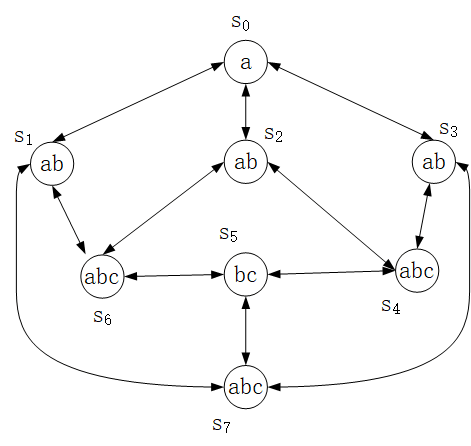
\includegraphics[width=0.4\textwidth]{k2.png}}
        \hspace{1in}
        \subfigure[$V$-quotient Kripke structure of $\Hm$]{
        \label{Kripke_2:VQ} %% label for second subfigure%
       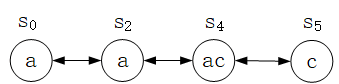
\includegraphics[width=0.3\textwidth]{k2VQ.png}}
       \caption{Computing the $V$-quotient Kripke structure}
    \label{fig:subfig} %% label for entire figure%
\end{figure}
\end{example}

Similar with the $V$-bisimulation between \MPK-structures, we define the $\tuple{V,I}$-bisimulation between \Ind-structures as follows:
\begin{definition}\label{def:VInd:bisimulation}
\textbf{($\tuple{V,I}$-bisimulation)}
Let $\Hm_i=(S_i, R_i, L_i, [\_]_i, s_i)$ with $i\in \{1, 2\}$ be two \Ind-structures, $V$ be a set of atoms and $I \subseteq Ind$. The $\tuple{V,I}$-bisimulation $\beta_{\tuple{V,I}}$ between \Ind-structures is a set that satisfy $((\Hm_1, s_1), (\Hm_2, s_2)) \in \beta_{\tuple{V,I}}$  if and only if:
\begin{enumerate}[(i)]
    \item $L_1(s_1) - V \equiv L_2(s_2) -V$;
    \item $\forall (s_1, s_1')\in R_1$, $\exists (s_2, s_2')\in R_2$ s.t. $((\Hm_1, s_1'), (\Hm_2, s_2')) \in \beta_{\tuple{V,I}}$;
    \item $\forall (s_2, s_2')\in R_2$, $\exists (s_1, s_1')\in R_1$ s.t. $((\Hm_1, s_1'), (\Hm_2, s_2')) \in \beta_{\tuple{V,I}}$;
    \item $\forall i \notin I$ there is $[i]_1 = [i]_2$.
\end{enumerate}
\end{definition}
Apparently, this definition is similar with our concept $V$-bisimulation except that this $\tuple{V,I}$-bisimulation has introduced the index.
Besides, it is not difficult to prove $\tuple{V,I}$-bisimulation possess those properties (talked-above) possessed by $V$-bisimulation.



\subsection{Characterize formula of initial \MPK-structure}
Given a set $V\subseteq\Ha$, we can define a formula $\varphi$ of $V$ (that is $\Var(\varphi) \subseteq V$) in \CTL\ to equivalent uniquely describe a computation tree.
\begin{definition}\label{def:V:char:formula}
Let $V\subseteq \Ha$, $\Hm =(S,R,L,s_0)$ be a model structure and $s\in S$.
The {\em characterize formula} of the computation tree $\Tr_n(s)$ on $V$,
written ${\cal F}_V(\Tr_n(s))$, is defined recursively as:
\begin{align*}
  & {\cal F}_V(\Tr_0(s)) = \bigwedge_{p \in V\cap L(s)}p
     \wedge \bigwedge_{q\in V-L(s)} \neg q,\\
  & {\cal F}_V(\Tr_{k+1}(s)) = \left(\bigwedge_{(s,s')\in R}
    \EXIST \NEXT {\cal F}_V(\Tr_k(s'))\right)
    \wedge \\
  & \qquad \qquad \ALL \NEXT\left(\bigvee_{(s,s')\in R}
    {\cal F}_V(\Tr_k(s') )\right)
    \wedge {\cal F}_V(\Tr_0(s))
\end{align*}
for $k\ge 0$.
\end{definition}
It is apparent that $\IR({\cal F}_V(\Tr_n(s)), \overline V)$.
As we will see that the characterize formula ${\cal F}_V(\Tr_n(s))$ equivalent uniquely describe the computation tree $\Tr_n(s)$ on $V$, that is for any formula $\varphi$ of $V$, if $\varphi$ is a characterize formula of $\Tr_n(s)$ then $\varphi \equiv {\cal F}_V(\Tr_n(s))$.


\begin{lemma}\label{Bn:to:Tn}
Let $V\subseteq \Ha$, $\Hm=(S, R, L,s_0)$ and $\Hm'=(S', R', L',s_0')$ be two model structures,
$s\in S$, $s'\in S'$ and $n\ge 0$.
\begin{enumerate}[(i)]
  \item $({\cal M},s)\models{\cal F}_V(\Tr_n(s))$.
  \item If $({\cal M},s)\models{\cal F}_V(\Tr_n(s'))$ then
  $\Tr_n(s) \lrto_{\overline V} \Tr_n(s')$.
\end{enumerate}
\end{lemma}


A consequence of the previous lemma is:

\begin{lemma}\label{div_s}
Let $V\subseteq \Ha$, $\Hm=(S,R,L,s_0)$ a model structure, $k={ch({\cal M},V)}$ and $s\in S$.
%There is a formula $\phi$ such that
\begin{itemize}
  \item $(\Hm, s)\models {\cal F}_V(\Tr_k(s))$, and
  \item for each $s'\in S$, $({\cal M},s) \lrto_{\overline V} ({\cal M},s')$
  if and only if $({\cal M},s')\models{\cal F}_V(\Tr_k(s))$.
\end{itemize}
\end{lemma}
\begin{proof}
Let $\phi = {\cal F}_V(\Tr_k(s))$, where $c$ is the V-characteristic number of $\Hm$. $\Hm, s \models \phi$ by the definition of ${\cal F}$, and then $\forall s' \in S$, if $s \lrto_{\overline V} s'$ there is $\Hm, s' \models \phi$ by Theorem~\ref{thm:V-bisimulation:EQ} due to $\IR(\phi, \Ha \setminus V)$. If $s \nleftrightarrow_{\overline V} s'$, then $\Tr_c(s) \not \lrto_{\overline V} \Tr_c(s')$, and then $\Hm, s\nvDash \phi$ by Lemma~\ref{Bn:to:Tn}.
\end{proof}



\begin{lemma}\label{lem:Vb:TrFormula:Equ}
Let $V\subseteq \Ha$, $\Hm=(S, R, L, s_0)$ and $\Hm'=(S', R', L', s_0')$ be two model structures,
$s\in S$, $s'\in S'$ and $n\ge 0$. If $\Tr_n(s) \lrto_{\overline V} \Tr_n(s')$, then ${\cal F}_V(\Tr_n(s)) \equiv {\cal F}_V(\Tr_n(s'))$.
\end{lemma}
%\begin{proof}
%This result can be proved by inducting on $n$.
%
%\textbf{Base.} It is apparent that for any $s_n\in S$ and $s_n' \in S'$, if $\Tr_0(s_n) \lrto_{\overline V} \Tr_0(s_n')$ then ${\cal F}_V(\Tr_0(s_n)) \equiv {\cal F}_V(\Tr_0(s_n'))$ due to $L(s_n) - \overline V = L'(s_n') - \overline V$ by known.
%
%\textbf{Step.} Supposing that for $k=m$ $(0< m < n)$ there is if $\Tr_{n-k}(s_k) \lrto_{\overline V} \Tr_{n-k}(s_k')$ then ${\cal F}_V(\Tr_{n-k}(s_k)) \equiv {\cal F}_V(\Tr_{n-k}(s_k'))$, then we will show if $\Tr_{n-k+1}(s_{k-1}) \lrto_{\overline V} \Tr_{n-k+1}(s_{k-1}')$ then ${\cal F}_V(\Tr_{n-k+1}(s_{k-1})) \equiv {\cal F}_V(\Tr_{n-k+1}(s_{k-1}'))$. Apparent that:\\
% ${\cal F}_V(\Tr_{n-k+1}(s_{k-1})) =$ \\
% $\left(\bigwedge_{(s_{k-1},s_k)\in R}
%    \EXIST \NEXT {\cal F}_V(\Tr_{n-k}(s_k))\right)
%    \wedge \ALL \NEXT\left(\bigvee_{(s_{k-1},s_k)\in R}
%    {\cal F}_V(\Tr_{n-k}(s_k) )\right)
%    \wedge {\cal F}_V(\Tr_0(s_{k-1}))$\\
% ${\cal F}_V(\Tr_{n-k+1}(s_{k-1}')) =$ \\
% $\left(\bigwedge_{(s_{k-1}',s_k')\in R}
%    \EXIST \NEXT {\cal F}_V(\Tr_{n-k}(s_k'))\right)
%    \wedge \ALL \NEXT\left(\bigvee_{(s_{k-1}',s_k')\in R}
%    {\cal F}_V(\Tr_{n-k}(s_k') )\right)
%    \wedge {\cal F}_V(\Tr_0(s_{k-1}'))$ by the definition of characterize formula of the computation tree.
% Then we have for any $(s_{k-1}, s_k) \in R$ there is $(s_{k-1}', s_k') \in R'$ such that $\Tr_{n-k}(s_k) \lrto_{\overline V} \Tr_{n-k}(s_k')$ by $\Tr_{n-k+1}(s_{k-1}) \lrto_{\overline V} \Tr_{n-k+1}(s_{k-1}')$. Besides, for any $(s_{k-1}', s_k') \in R'$ there is $(s_{k-1}, s_k) \in R$ such that $\Tr_{n-k}(s_k) \lrto_{\overline V} \Tr_{n-k}(s_k')$ by $\Tr_{n-k+1}(s_{k-1}) \lrto_{\overline V} \Tr_{n-k+1}(s_{k-1}')$.
% Therefore, we have ${\cal F}_V(\Tr_{n-k+1}(s_{k-1})) \equiv {\cal F}_V(\Tr_{n-k+1}(s_{k-1}'))$ by induction hypothesis.
%\end{proof}
Let $s'=s$, this show that for any formula $\varphi$ of $V$, if $\varphi$ is a characterize formula of $\Tr_n(s)$ then $\varphi \equiv {\cal F}_V(\Tr_n(s))$.



Let $V\subseteq\cal A$, ${\cal M}=(S,R,L,s_0)$
and ${\cal K}=({\cal M},s_0)$ be an initial \MPK-structure.
The {\em characterizing formula} of $\cal K$ on $V$, written ${\cal F}_V(\Hm,s_0)$ (or ${\cal F}_V({\cal K})$), is
defined as the conjunction of the following formulas:
\begin{align*}
  &{\cal F}_V(\Tr_c(s_0)), \mbox{ and }\\
%  &  \bigwedge_{s\in S}\left(
  & \ALL \GLOBAL\left(
    {\cal F}_V(\Tr_c(s)) \rto
    \bigwedge_{(s,s')\in R}
        \EXIST \NEXT {\cal F}_V(\Tr_c(s'))
        \wedge
        \ALL \NEXT \bigvee_{(s,s')\in R}{\cal F}_V(\Tr_c(s'))
    \right) \\
  & \qquad  \qquad \qquad ,\ s\in S
\end{align*}
%\begin{equation*}
%\resizebox{.91\linewidth}{!}{$
%\displaystyle
%\ALL \GLOBAL\left(
%    {\cal F}_V(\Tr_c(s)) \rto
%    \bigwedge_{(s,s')\in R}
%        \EXIST \NEXT {\cal F}_V(\Tr_c(s'))
%        \wedge
%        \ALL \NEXT \bigvee_{(s,s')\in R}{\cal F}_V(\Tr_c(s'))
%    \right), \ s\in S
%$}
%\end{equation*}
where $c=ch({\cal M},V)$. It is apparent that $\IR({\cal F}_V(\Hm, s_0), \overline V)$.


\begin{lemma}\label{lem:models:formula}
  Let $\varphi$ be a formula. We have
  \begin{equation}
    \varphi\equiv \bigvee_{(\Hm, s_0)\in\Mod(\varphi)}{\cal F}_{\cal A}(\Hm, s_0).
\end{equation}
\end{lemma}

This means that any \CTL\ formula can be described by the disjunction of the characterizing formulas of all the models of itself due to the number of models of a \CTL\ formula is finite.

\begin{theorem}\label{CF}
Let $V\subseteq \Ha$, $\Hm=(S,R,L,s_0)$ be a model structure with initial state $s_0$
and $\Hm'=(S',R', L',s_0')$ be a model structure with initial state $s_0'$.
Then  $$(\Hm',s_0') \models {\cal F}_V({\cal M},s_0)
\mbox{ if and only if }
({\cal M},s_0) \lrto_{\overline V} ({\cal M}',s_0').$$
\end{theorem}

We will give an example to show the computing of characterizing formula:
\begin{example}
Let ${\cal K} = (\Hm, s_0)$ with $\Hm=(S, R, L,s_0)$ be a initial \MPK-structure (in Fig.~\ref{Kripke_1}), in which $S=\{s_0, s_1, s_2\}$, $R=\{(s_0, s_1), (s_0, s_2), (s_1, s_0), (s_2, s_0)\}$, $L(s_0)= \{a\}$, $L(s_1) =\{a,c\}$ and $L(s_2) = \{b,c\}$. Let $V=\{a, b\}$, compute the characterizing formula of ${\cal K}$ on $V$.

It is apparent that $\Tr_0(s_0) \lrto_{\overline V} \Tr_0(s_1)$ due to $L(s_0) - \overline V = L(s_1) -\overline V$, $\Tr_1(s_0) \not\lrto_{\overline V} \Tr_1(s_1)$ due to there is $(s_0, s_2)\in R$ such that for any $(s_1, s') \in R$ (there is only one immediate successor $s'=s_0$) there is $L(s_2) - \overline V \neq L(s') - \overline V$. Hence, we have that $\Hm$ is $\overline V$-distinguished by state $s_0$ and $s_1$ at the least depth 1, \ie\ $\dis_{\overline V}(\Hm, s_0, s_1, 1)$. Similarly, we have $\dis_{\overline V}(\Hm, s_0, s_2, 0)$ and $\dis_{\overline V}(\Hm, s_1, s_2, 0)$. Therefore, $ch(\Hm, \overline V) =  \max\{k\mid s,s'\in S\ \&\ \dis_{\overline V}({\cal M},s,s',k)\} = 1$.
%It is apparent that $\Hb_0=\{(s_0, s_1)\}$ and $\Hb_1={\O}$, then $ch(\Hm, s_0) = 1$.
Then we have:
\begin{align*}
  & {\cal F}_V(\Tr_0(s_0)) = a \wedge \neg b, \\
  & {\cal F}_V(\Tr_0(s_1)) = a \wedge \neg b, \\
  & {\cal F}_V(\Tr_0(s_2)) = b \wedge \neg a, \\
  & {\cal F}_V(\Tr_1(s_0)) = \EXIST\NEXT(a \wedge \neg b)  \wedge \EXIST\NEXT(b \wedge \neg a) \wedge \ALL\NEXT((a \wedge \neg b) \vee\\
  & \qquad \qquad  \qquad (b \wedge \neg a)) \wedge (a \wedge \neg b), \\
  & {\cal F}_V(\Tr_1(s_1)) = \EXIST\NEXT(a \wedge \neg b)  \wedge \ALL\NEXT(a \wedge \neg b) \wedge (a \wedge \neg b), \\
  & {\cal F}_V(\Tr_1(s_2)) = \EXIST\NEXT(a \wedge \neg b)  \wedge \ALL\NEXT(a \wedge \neg b) \wedge (b \wedge \neg a).\\
  & \mbox{ Then it is easy to obtain\ } {\cal F}_V(\Hm, s_0).
  %&{\cal F}_V(\Hm, s_0)= {\cal F}_V(\Tr_1(s_0)) \wedge  \bigwedge_{s\in S} \ALL \GLOBAL \left(
%  {\cal F}_V(\Tr_1(s)) \rto
%  \bigwedge_{(s,s')\in R}
%        \EXIST \NEXT {\cal F}_V(\Tr_1(s'))
%        \wedge
%        \ALL \NEXT \bigvee_{(s,s')\in R}{\cal F}_V(\Tr_1(s'))
%  \right)
\end{align*}

\begin{figure}
  \centering
  % Requires \usepackage{graphicx}
  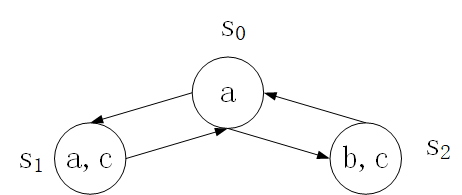
\includegraphics[width=5cm]{k1.png}\\
  \caption{A simple Kripke structure}\label{Kripke_1}
\end{figure}
\end{example}

By the following theorem we also have that given a set $V\subseteq \Ha$, the characterizing formula of an initial \MPK-structure is equivalent uniquely describe this initial \MPK-structure on $V$.
\begin{theorem}\label{thm:VBChFEQ}
Let $V\subseteq \Ha$, $\Hm=(S,R,L,s_0)$ a model structure with initial state $s_0$
and $\Hm'=(S',R', L',s_0')$ a model structure with initial state $s_0'$.
If $({\cal M},s_0) \lrto_{\overline V} ({\cal M}',s_0')$ then ${\cal F}_V(\Hm, s_0) \equiv {\cal F}_V(\Hm', s_0')$.
\end{theorem}
\begin{proof}
This is following Lemma~\ref{lem:Vb:TrFormula:Equ} and the definition of the characterizing formula of initial \MPK-structure ${\cal K}$ on $V$.
\end{proof}


\subsection{Forgetting on CTL}
Having talked about the $V$-bisimulation between two \MPK-structures and the characterizing formula of a \MPK-structure, we will give the definition of forgetting under CTL from the sematic forgetting point of view.
\begin{definition}[Forgetting]\label{def:V:forgetting}
  Let $V\subseteq\cal A$ and $\phi$ a formula.
A formula $\psi$ with $\Var(\psi)\cap V=\emptyset$
is a {\em result of forgetting $V$ from} $\phi$, if
\begin{equation}
\resizebox{.91\linewidth}{!}{$
\displaystyle
  \Mod(\psi)=\{{\cal K}\mbox{ is initial}\mid \exists {\cal K}'\in\Mod(\phi)\ \&\ {\cal K}'\lrto_V{\cal K}\}.
  $}
\end{equation}
\end{definition}
Note that if both $\psi$ and $\psi'$ are results of forgetting $V$ from $\phi$ then
$\Mod(\psi)=\Mod(\psi')$, \ie, $\psi$ and $\psi'$ have the same models. In the sense
of equivalence the forgetting result is unique (up to equivalence).
By Lemma~\ref{lem:models:formula}, such a formula $\psi$ always exists, which
is equivalent to
\begin{equation*}
\resizebox{.91\linewidth}{!}{$
\displaystyle
  \bigvee_{{\cal K}\in  \{{\cal K}'\mbox{ is an initial interpretation}\mid \exists {\cal K}''\in\Mod(\phi)\ \&\ {\cal K}''\lrto_V{\cal K}'\}} {\cal F}_{\overline V}({\cal K}).
  $}
\end{equation*}
For this reason, the forgetting result is denoted by $\CTLforget(\phi,V)$. By the definition of forgetting, we have

\begin{proposition}\label{pro:IR_V:forget}
Let $\varphi$ be a CTL formula and $V$ a set of atoms. If $V \cap \Var(\varphi) = {\O}$, then
\[
\CTLforget(\varphi,V) \equiv \varphi.
\]
\end{proposition}
\begin{proof}
 $(\Rto)$ $\forall (\Hm, s_0) \in \Mod(\CTLforget(\varphi,V))$ \\ $\Rto$ there is $(\Hm', s_0')$ s.t. $(\Hm', s_0')\lrto_V (\Hm, s_0)$ and $(\Hm', s_0') \models \varphi$ \\
 $\Rto$ $(\Hm, s_0) \models \varphi$ \hfill ($\IR(\varphi, V)$)\\

 $(\Lto)$ $\forall (\Hm, s_0)\in \Mod(\varphi)$ there is $(\Hm, s_0) \models \CTLforget(\varphi, V)$ by $(W)$.
\end{proof}

In the case $\psi$ is a result of forgetting $V$ from $\phi$, there are usually some
expected properties (called {\em postulates}) for them~\cite{Yan:AIJ:2009}:
\begin{itemize}
  \item Weakening (\W): $\varphi \models \psi$;
  \item Positive Persistence (\PP):
    if $\IR(\eta, V)$ and $\varphi \models \eta$, then $\psi \models \eta$;
  \item Negative Persistence (\NgP): if $\IR(\eta, V)$ and $\varphi \nvDash \eta$, then $\psi \nvDash \eta$;
  \item Irrelevance (\textbf{IR}): $\IR(\psi, V)$.
\end{itemize}


\begin{theorem}\label{thm:close}
Let $\varphi$ and $\psi$ be two formulas and $V \subseteq \Ha$.
Then the following statements are equivalent:
\begin{enumerate}[(i)]
  \item $\psi \equiv \CTLforget(\varphi, V)$,
  \item $\psi \equiv \{\phi | \varphi \models \phi \& \IR(\phi, V)\}$,
  \item Postulates (\W), (\PP), (\NgP) and (\textbf{IR}) hold.
\end{enumerate}
\end{theorem}
We can see from this theorem that the forgetting under CTL is closed, \ie\ for any CTL formula the result of forgetting is also a CTL formula.


\begin{lemma}\label{lem:KF:eq}
	Let $\varphi$ and $\alpha$ be two \CTL\ formulae and $q\in
		\overline{\Var(\varphi\cup\{\alpha\})}$. Then
	$\forget(\varphi \cup\{q\lrto\alpha\}, q)\equiv \varphi$.
\end{lemma}


\begin{proposition}\label{disTF}
Let $\varphi$ be a formula, $V$ a set of atoms and $p$ an atom such that $p \notin V$. Then:
\[
\CTLforget(\varphi, \{p\} \cup V) \equiv \CTLforget(\CTLforget(\varphi, p), V).
\]
\end{proposition}
This means that the result of forgetting $V$ from $\varphi$ can be obtained by forgetting atom in $V$ one by one.
Similarly, a consequence of the previous proposition is:

\begin{corollary}\label{disTFV}
Let $\varphi$ be a formula and $V_i\subseteq{\cal A}~(i=1,2)$. Then:
\[
\CTLforget(\varphi, V_1 \cup V_2) \equiv \CTLforget(\CTLforget(\varphi, V_1), V_2).
\]
\end{corollary}



The following results, which are satisfied in both classical proposition logic and modal logic \SFive, further illustrate other essential semantic properties of forgetting.
\begin{proposition}\label{pro:ctl:forget:1}
Let $\varphi$, $\varphi_i$, $\psi_i$ ($i=1,2$) be formulas and $V\subseteq \Ha$. We have
\begin{enumerate}[(i)]
  \item $\CTLforget(\varphi, V)$ is satisfiable iff $\varphi$ is;
  \item If $\varphi_1 \equiv \varphi_2$, then $\CTLforget(\varphi_1, V) \equiv \CTLforget(\varphi_2, V)$;
  \item If $\varphi_1 \models \varphi_2$, then $\CTLforget(\varphi_1, V) \models \CTLforget(\varphi_2, V)$;
  \item $\CTLforget(\psi_1 \vee \psi_2, V) \equiv \CTLforget(\psi_1, V) \vee \CTLforget(\psi_2, V)$;
  \item $\CTLforget(\psi_1 \wedge \psi_2, V) \models \CTLforget(\psi_1, V) \wedge \CTLforget(\psi_2, V)$.
\end{enumerate}
\end{proposition}


Another interest result is that the forgetting of the fragment $P T \varphi$ ($P\in \{\EXIST, \ALL\}$, $T \in \{\FUTURE, \NEXT\}$) on $V\subseteq \Ha$ can be computed by $PT \CTLforget(\varphi, V)$. This give a convenient method to compute forgetting.
\begin{proposition}\label{pro:ctl:forget:2}
  Let $V\subseteq\cal A$ and $\phi$ a formula.
  \begin{enumerate}[(i)]
    \item $\CTLforget(\ALL\NEXT\phi,V)\equiv\ALL\NEXT \CTLforget(\phi,V)$.
    \item $\CTLforget(\EXIST\NEXT\phi,V)\equiv\EXIST\NEXT \CTLforget(\phi,V)$.
    \item $\CTLforget(\ALL\FUTURE\phi,V)\equiv\ALL\FUTURE \CTLforget(\phi,V)$.
    \item $\CTLforget(\EXIST\FUTURE\phi,V)\equiv\EXIST\FUTURE \CTLforget(\phi,V)$.
  \end{enumerate}
\end{proposition}



\section{Algorithm to compute forgetting}
To compute the forgetting in \CTL, we propose two methods, model-based and resolution-based, in this part.
Literally speaking, the model-based method means that we can obtain the result of forgetting in \CTL\ by obtain all the possible finite \MPK-models of this result. How can we obtain all the \MPK-models is what we will solved in this part.
The resolution-based method obtain the result of forgetting by obtaining all the possible resolutions which can be implied by the original formula.

However, the resolution-based method is different from that in CPL~\cite{Yisong:2015:arx} due to it is easy to transform any CPL formula into a CNF.
However, it is difficult to transform a \CTL\ formula into a form similar with CNF in \CTL.
Fortunately, there is an extension of \CTL\ such that any \CTL\ formula can be transformed into the extension in polynomial time.
And we will give a detailed description later. Before that,  let turn to the model-based method at first.
\subsection{A model-based algorithm}
As we have said that the set models of any formula $\varphi$ is finite, hence if we can obtain all the models of $\varphi$ then we can express this formula by the disjunction of those characteristic formulas of those models.
By the definition of forgetting in \CTL, the set of models of the result of forgetting is a finite set of initial \MPK-structures.
Then the model-based method is generated for forgetting in \CTL.

Though the set of models of the result of forgetting is finite, while how many models is there?
That's right we should given the bound of the number of the models.
As it is said in Proposition-- that if two initial \MPK-structures are $V$-bisimulation, then their characteristic formulas is equal.
Then let $\varphi$ be a CTL formula, the $|\Var(\varphi)|=m$ is a positive integer, we have the following theorem:
\begin{theorem}
Let $\varphi$ be a CTL formula, $V=\Var(\varphi)$, $|V|=m$, and ${\cal K}=(\Hm, s_0)$ with $\Hm=(S, R,L,s_0)$ be a initial \MPK-structure. If $(\Hm, s_0) \models \varphi$, then there is an initial \MPK-structure ${\cal K}'=(\Hm', s_0')$ with $\Hm'=(S', R',L',s_0')$ that satisfy:
\begin{enumerate}[(i)]
  \item $|S'|$ is at most $2^m$,
  \item $|R'|$ is at most $2^m * 2^m$,
  \item $|L'|$ is at most $2^m * 2^m$,
  \item ${\cal K} \lrto_{\Ha \setminus V} {\cal K}'$ and $(\Hm', s_0') \models \varphi$.
\end{enumerate}
\end{theorem}
\begin{proof}
If $|S| \leq 2^m$, this result clearly holds. If $|S| > 2^m$, let ${\cal K}' = {\cal K}_{|V}$, then it is apparent that ${\cal K} \lrto_{\Ha \setminus V} {\cal K}'$ by Proposition~\ref{pro:VQ} and $(\Hm', s_0') \models \varphi$. In the worst case, the number of states in $S'$ is $2^m$ by the definition of ${\cal K}_{|V}$. Then the theorem is proved.
\end{proof}

By this theorem, we can see that any initial \MPK-structures ${\cal K}$ that satisfy $\varphi$ can be transformed to an initial \MPK-structure ${\cal K}'$ such that ${\cal K} \lrto_{\Ha \setminus V} {\cal K}'$ and ${\cal K} \models \varphi$ iff ${\cal K}' \models \varphi$ due to $\IR(\varphi, \Ha\setminus V)$, in which $V= \Var(\varphi)$. Therefore, the size of the model of $\varphi$ is at most $2^m$ by Theorem~\ref{thm:VBChFEQ}(we only consider the number of states of this model).

Then we have the following model-based Algorithm~\ref{alg:compute:forgetting:by:VB} to computing the forgetting under CTL:


\begin{algorithm}
\caption{Model-based: Computing forgetting}
\label{alg:compute:forgetting:by:VB}
\KwIn{A CTL formula $\varphi$ and a set $V$ of atoms}
\KwOut{$\CTLforget(\varphi, V)$}% ????
$T={\O}$ // the set of models of $\varphi$ \;
$T' = {\O}$ // the set of models of $\CTLforget(\varphi, V)$ \;
$m=|\Var(\varphi)|$\;
$n=|V|$\;

\For {i=1, ..., $2^m$}{
        Enumerating all possible initial \MPK-structures $(\Hm, s_0)$ with $\Hm=(S, R, L,s_0)$ and $|S|=i$\;
        For all initial \MPK-structures $(\Hm, s_0)$ \If {$(\Hm,s_0) \models \varphi$}{
            $T= T \cup \{(\Hm,s_0)\}$\;
        }
}
\For {${\cal K} =(\Hm, s_0) \in T$} {
    Let $T' = T' \cup \{{\cal K}_{|V} \}$\;
}

\For {i=1, ..., $2^{m-n}$}{
        Enumerating all possible initial \MPK-structures $(\Hm', s_0')$ with $\Hm'=(S', R', L',s_0')$ and $|S'|=i$\;
        For all initial \MPK-structures $(\Hm', s_0')$ \If {$\exists (\Hm,s_0)\in T$ s.t. $(\Hm,s_0) \lrto_V (\Hm', s_0')$}{
            $T'= T' \cup \{(\Hm',s_0')\}$\;
        }
}
\Return $\bigvee_{(\Hm', s_0')\in T'} {\cal F}_{\overline V}(\Hm', s_0')$.
\end{algorithm}


\begin{proposition}
 Let $\varphi$ be a CTL formula and $V\subseteq \Ha$. The time complexity of
Algorithm~\ref{alg:compute:forgetting:by:VB} is $O(2^{2^m})$ and the space complexity is $O(2^{2m})$. Where $|Var(\varphi)| = m$ and $|V| = n$.
\end{proposition}
\begin{proof}
The time and space spend by Algorithm~\ref{alg:compute:forgetting:by:VB} is mainly the \textbf{for} cycles from sentence 5 to 10.
Under a given number $i$ of states, there are $i^i$ number of relations, $i^m$ number of label functions and $i$ number of possible initial states. In the case, we need the memory for the initial \MPK-model in each time is $(i+i^2+i*m+1)$.
Therefore, in the worst case is $i=2^m$, that is we need $(2^m + 2^{2m}+m*2^m+1)$ memory to store the initial \MPK-model.

For the time complexity, for each $1\leq i \leq 2^m$, there is at most $i*i^i*i^m*i=i^2*2^{(i+m)}$ possible initial \MPK-models.
If we suppose that we can obtain an initial \MPK-models in unit time, then in there will spend $(2^m)^2*2^{2^m+m}$ unit time in the worst case. Therefore, the time complexity is $O(2^{2^m})$.
\end{proof}




\subsection{A resolution-based algorithm}
As said above that the time complexity of the model-based method is $O(2^{2^m})$, it is crazy even for $m=4$. Dose there is an efficient time to do this work? The answer is yes! In this part, we will explore a resolution-based method to compute forgetting in \CTL. In this part we use the transformation rules Trans(1) to Trans(12) and resolution rules $\textbf{(SRES1)}, \dots, \textbf{(SRES8)}, \textbf{RW1}, \textbf{RW2}, \textbf{(ERES1)}, \textbf{(ERES2)}$ in~\cite{zhang2009refined}.

The main idea of this method is made up of three parts: (1) Transform a \CTL\ formula $\varphi$ into a set $T_{\varphi}$ of $\CTLsnf$ clauses; (2) Do all the possible resolutions on the set $V$ of atoms we want to forget and the set $V'$ introduced in (1); and (3) Eliminate those clauses that include at least one atom in $V\cup V'$. For (1) and (2) there are two good literals~\cite{bolotov2000clausal,zhang2009refined} to do it.
In this paper we resolve the problem (3) and the problem of how to compute forgetting in \CTL\ with the resolution in \CTL\ with index.
 As we will see that the $\tuple{V,I}$-bisimulation relation set up a bridge for \CTL\ and $\CTLsnf$ language.

 \begin{proposition}\label{pro:Elim:start}
Let $\varphi$, $P$, $C$ and $D$ be four formulae, where $m_j$ $(1\leq j \leq k)$ are literals. Then
\begin{enumerate}[(i)]
    \item $\varphi \equiv \ALL \GLOBAL (\start \supset \varphi)$,
    \item $P \supset C \vee D \equiv \ALL \GLOBAL (\start \wedge P \supset C \vee D)$.
\end{enumerate}
%Where $P$ is a conjunction of literals, $C$ are disjunction of literals. (P, C, D are any formula)
\end{proposition}
Which means that we can change a set of $\CTLsnf$ to another set without $\start$.

Let $T$ be a set of $\CTLsnf$ clauses, we define $T'$, called \emph{nonInd}-$\CTLsnf$, as follows:
\begin{align*}
& T' = \{C'| C' =P\supset \EXIST \daleth D\ \mbox{if}\ C = P\supset \EXIST_{\tuple{ind}}\daleth D \\
& \text{else}\ C' = C,\  C\in T, \daleth\in \{\NEXT, \FUTURE\}\}.
\end{align*}

\begin{lemma}\label{lem:No:Ind}
\textbf{(NI-BRemain)}
Let $T$ be a set of $\CTLsnf$ clauses and $T'$ be the nonInd-$\CTLsnf$ of $T$.
Then we have $T \equiv_{\tuple{{\O}, I}} T'$,
%Then $\forall (\Hm,s_0) \in \Mod(T)$ there is a $(\Hm',s_0') \in \Mod(T')$ such that $(\Hm,s_0) \lrto_{\tuple{{\O}, I}} (\Hm',s_0')$ and vice versa.
where $I$ is the set of indexes in $T$.
\end{lemma}

Similarly, let $T$ be a set of $\CTLsnf$ clauses, then we define the following operator:
\begin{align*}
&T_{\CTL} = \{C|C'\in T'\ \mbox{and}\ C = D \ \mbox{if}\ C' \in T\\
& \mbox{is the form}\ \ALL\GLOBAL(\start\supset D), \mbox{else}\ C= C'\}.
\end{align*}
It is obvious that $T' \equiv T_{\CTL}$ by Proposition~\ref{pro:Elim:start}.



The transformation of an arbitrary CTL formula into the set $T_{\varphi}$ start with the set $T_0=\{\ALL \GLOBAL(\start \supset p), \ALL \GLOBAL(p \supset \simp(\nnf(\varphi)))\}$ (it has proved that $\simp(\nnf(\varphi)) \equiv \varphi$~\cite{bolotov2000clausal}), where $p$ is a new proposition that dose not occur in $\varphi$, $\nnf$ is a function that transforms an arbitrary CTL formula into its negation normal form (NNF) by pushing negations inwards and $\simp$ is a function simplifies an arbitrary CTL formula by simplification rules~\cite{zhang2009refined}. And then construct a sequence $T_0, T_1,\dots, T_n=T_{\varphi}$ of formulea such that for every $i$ ($0 \leq i< n$), $T_{i+1} = (T_i \setminus \{\psi\}) \cup R_i$, where $\psi$ is a formula in $T_i$ not in $\CTLsnf$ clause and $R_i$ is the result set of applying a matching transformation rule to $\psi$. Besides, throughout the transformation formulae are kept in NNF.
Let $T$, $T'$ be two set of formulae, $I$ a set of indexes and $V\subseteq \Ha$, by $T\equiv_{\tuple{V, I}} T'$ we mean that $\forall (\Hm, s_0) \in \Mod(T)$ there is a $(\Hm', s_0')$ such that $(\Hm,s_0) \lrto_{\tuple{V, I}} (\Hm',s_0')$ and $(\Hm', s_0') \models T'$ and vice versa.
Then we have:

\begin{lemma}\label{lem:T_0}
\textbf{(T0-VIB)}
Let $\varphi$ be a CTL formula, then $\varphi \equiv_{\tuple{\{p\}, {\O}}} T_0$.
\end{lemma}
\begin{proof}
 $(\Rto)$ $\forall (\Hm_1,s_1) \in \Mod(\varphi)$, \ie $(\Hm_1,s_1) \models \varphi$. We can construct an \Ind-model structure $\Hm_2$ is identical to $\Hm_1$ except $L_2(s_2) = L_1(s_1) \cup \{p\}$. It is apparent that $(\Hm_2,s_2) \models T_0$ and $(\Hm_1, s_1) \lrto_{\tuple{\{p\}, {\O}}} (\Hm_2, s_2)$.

 $(\Lto)$ $\forall (\Hm_1,s_1) \in \Mod(T_0)$, it is apparent that $(\Hm_1,s_1) \models \varphi$ by the sematic of $\start$.
\end{proof}

By $\psi \rto_t R_i$ we mean using transformation rules $t$ on formula $\psi$ (the formulae $\psi$ as the
premises of rule $t$) and obtaining the set  $R_i$ of transformation results. Let $X$ be a set of formulas
we have the following result.
\begin{lemma}\label{lem:Trans(1)}
If $\psi \rto_t R_i$ by an application of $t\in \{$Trans(1), $\dots$, Trans(12)$\}$, then $T_i \equiv_{\tuple{\{p\}, \{ind\}}} T_{i+1}$.
Where $T_i= X \cup \{\psi\}$, $T_{i+1}=X \cup R_i$ and $p$ (if any), $ind$ (if any) are the atom and index introduced by using that rule respectively.
\end{lemma}

\begin{proposition}\label{pro:Tran:VIB}
Let $\varphi$ be a CTL formula, then we have $\varphi \equiv_{\tuple{V, I}} T_{\varphi}$.
Where $V$ be a set of new propositions introduced in the process of translate $\varphi$ into $T_{\varphi}$, and $I$ be the set of index appearing in $T_{\varphi}$.
\end{proposition}
\begin{proof}
This can be proved from Lemma~\ref{lem:T_0} and Lemma~\ref{lem:Trans(1)}.
\end{proof}





A \emph{derivation} on a set $V$ of atoms from a set $T$ of $\CTLsnf$ clauses by using those resolution rules in~\cite{zhang2009refined} on $V$ (\ie do resolutions only on the atoms in $V$) is a sequence $T_0, T_1, T_2$, $\dots$, $T_n=T^{r,V}$ of sets of $\CTLsnf$ clauses such that $T = T_0$ and $T_{i+1} = T_i \cup R_i$ where $R_i$ is a set of clauses obtained as the conclusion of the application of a resolution rule to premises in $T_i$. And we call $T^{r,V}$ is the result of resolution of $T$ on $V$ by using resolution rules.
Besides, if there is a $T_i$ containing $\start\supset \perp$ or $\top\supset \perp$, then $T_i$ is unsatisfiable and then $\varphi$ is unsatisfiable. In this case we do not need to compute other $T_j$  ($j> i$).
By $\psi \rto_r R_i$ we mean using resolution rules $r$ on set $\psi$ (the formulae in $\psi$ as the premises of rule $r$) and obtaining the set $R_i$ of resolution results. For resolution rules, we have the following results.

\begin{lemma}\label{lem:SRES}
If $\psi \rto_r R_i$ by an application of $r\in \{\textbf{(SRES1)}, \dots, \textbf{(SRES8)}, \textbf{RW1}, \textbf{RW2}\}$,
then $T_i \equiv_{\tuple{\{p\}, {\O}}} T_{i+1}$.
Where $T_i= X \cup \psi$, $T_{i+1}=X \cup R_i$, $p$ be the proposition corresponding with literal $l$ used to do resolution in $r$.
\end{lemma}
\begin{proof}
On one hand, it is apparent that $\psi \models R_i$ and then $T_i \models T_{i+1}$. On the other hand, $T_i\subseteq T_{i+1}$ and then $T_{i+1} \models T_i$.
\end{proof}

\begin{lemma}\label{lem:ERES1}
If $\psi \rto_r R_i$ by an application of $r=$\textbf{(ERES1)},
then $T_i \equiv_{\tuple{\{l, w_{\neg l}^{\ALL}\}, {\O}}} T_{i+1}$.
Where $T_i= X \cup \psi$, $T_{i+1}=X \cup R_i$, $p$ be the proposition corresponding with literal $l$ used to do resolution in $r$.
\end{lemma}
\begin{proof}
 It has been proved that $\psi \models R_i$ in~\cite{bolotov2000clausal}, then there is $T_{i+1}=T_i \cup \Lambda_{\neg l}^{\ALL}$ and  then $\forall (\Hm_1,s_1) \in \Mod(T_i= X \cup \psi)$ there is a $(\Hm_2, s_2)\in \Mod(T_{i+1}=T_i \cup \Lambda_{\neg l}^{\ALL})$ s.t. $(\Hm_1, s_1) \lrto_{\tuple{\{p, w_{\neg l}^{\ALL}\}, {\O}}} (\Hm_2, s_2)$ and vice versa by Proposition~\ref{pro:Tran:VIB}.
\end{proof}
For rule \textbf{(ERES2)} we have the same result.

\begin{proposition}
Let $\varphi$ be a CTL formula and $V$ be a set of atoms, then we have $T_{\varphi} \equiv_{\tuple{V \cup V', {\O}}} T_{\varphi}^{r,V \cup V'}$.
Where $V'$ be a set of new propositions introduced in the process of transformation.
\end{proposition}
\begin{proof}
This is apparent from Lemma~\ref{lem:SRES} and Lemma~\ref{lem:ERES1}.
\end{proof}

Let $\varphi$ be a \CTL\ formula, $V \subseteq \Var(\varphi)$ be set of atoms and $V'$ be a set of new propositions introduced in the process of translate $\varphi$ into $T_{\varphi}$. By the transform and resolution rules, we have the following several important properties:
\begin{itemize}
  \item \textbf{(GNA)} for all atom $p$ in $\Var(\varphi)$, $p$ do not positively appear in the left hand of the $\CTLsnf$ clause;
  \item \textbf{(CNI)} for each global clause, there must be a atom $p\in V'$ appearing in the right hand negatively;
  \item \textbf{(PI)} for each atom $p\in V'$, if $p$ appearing in the left hand of a $\CTLsnf$ clause, then $p$ is positively.
\end{itemize}


A key point to compute forgetting is eliminate those irrelevant atoms, for this purpose, we define the follow substitution to find out those atoms that do irrelevant. A \emph{instantiate formula} of set $V$ of atoms is a formula that the atoms in $V$ do not appear in it.
%\begin{definition}\label{def:subst}
%[substitution] Let $\varphi$ be a \CTL\ formula, $V \subseteq \Var(\varphi)$ be a set of atoms and $V'$ be a set of new propositions introduced in the process of translating $\varphi$ into $T_{\varphi}$. The substitution of $((T_{\varphi}^{r,V \cup V'})')_{CTL}$ is that replace all the atoms $p$ in $V'$ by the formula $\psi$ that irrelevant with $V\cup V'$, we call it instantiate formula, if $p\supset \psi$, denoted as $\Sub((T_{\varphi}^{r,V \cup V'})', V)$.
%\end{definition}

\begin{definition}\label{def:subst}
%For convenience, we transform a global clause into a proper implication (the left hand only conclude atoms in $V'$).
[substitution] Let $\varphi$ be a \CTL\ formula, $V \subseteq \Var(\varphi)$ be a set of atoms and $V'=V'' \subseteq \Ha$ be a set of new propositions introduced in the process of translating $\varphi$ into $T_{\varphi}$. Let $\Gamma=(T_{\varphi}^{r,V \cup V'})'$, then the process of substitution is as follows:
\begin{enumerate}[(i)]
  \item for each global clause $C= \top \supset D \vee \neg p \in \Gamma$, if there is one and on one atom $p=\Var(l) \in V''\cap \Var(D)$  and $\Var(D) \cap V = {\O}$ then let $C = p \supset D$ and $V'':=V''\setminus \{p\}$;
  \item find out all the possible instantiate formulae $\varphi_1, ..., \varphi_m$ of $V \cup V''$ in the $p\supset \varphi_i \in \Gamma$ ($1\leq i\leq m$);
  \item if there is $p\supset \varphi_i$ for some $i\in \{1,\dots, m\}$, then let $V'':=V''\setminus \{p\}$, which means $p$ is a instantiate formula;
  \item for $\bigwedge_{j=1}^m p_j \supset \varphi_i \in \Gamma$ ($i\in \{1,\dots, m\}$), if there is $\alpha \supset p_1,\dots, \alpha \supset p_m \in \Gamma$ then let $\Gamma' := \Gamma \cup \{\alpha \supset \varphi\}$, if $\Gamma'\neq \Gamma$ then let $\Gamma:=\Gamma'$ return to (i);
  \item for $p\supset \varphi_{j_1}, \dots, p \supset \varphi_{j_n}\in \Gamma$, $j_i \in \{1,\dots, m\}$ then replace all $p$ in $\Gamma$ with $\bigwedge_{i=1}^{j_n} \varphi_{j_i}$, where $p$ do not appear in $\varphi_{j_i}$.
\end{enumerate}
Where $p, p_i$ ($1 \leq i\leq m$) are atoms and $\alpha$ is a conjunction of literals or $\start$.
\end{definition}

We denote this process as $\Sub(\Gamma, V')$. It is apparent that $(T_{\varphi}^{r,V \cup V'})' \equiv_{\tuple{V',{\O}}} \Sub((T_{\varphi}^{r,V \cup V'})',V')$.
\begin{example}\label{exa:until:sub}
Let $\varphi=\ALL((p\wedge q) \UNTIL (f\vee m)) \wedge r$ and $V=\{p\}$. Then we can compute $\Sub((T_{\varphi}^{r,V \cup V'})', V)$ as follows:

At first, we transform $\varphi$ into a set of $\CTLsnf$ with $V'=\{x,y,z\}$, which is listed as:
\begin{align*}
& 1. \start\supset z && 2. \top \supset \neg z \vee r && 3.\top \supset \neg x\vee f \vee m\\
& 4. \top \supset \neg z \vee x \vee y && 5.\top \supset \neg y \vee p && 6.\top \supset \neg y \vee q\\
& 7. z \supset \ALL \FUTURE x && 8. y \supset \ALL \NEXT(x\vee y).
\end{align*}

In the second, we compute all the possible resolution on $V\cup V'$,
\begin{align*}
&(1) \start \supset r && (1,2,SRES 5)\\
&(2) \start \supset x \vee y && (1,4,SRES 5)\\
&(3) \top \supset \neg z \vee y \vee f \vee m && (3, 4, SRES 8)\\
&(4) y \supset \ALL\NEXT(f\vee m\vee y) && (3,8, SRES 6)\\
&(5) \top \neg z \vee x \vee p && (4,5, SRES 8)\\
&(6) \top \neg z \vee x \vee q && (4,6, SRES 8)\\
&(7) y \supset \ALL\NEXT(x\vee p) && (5, 7, SRES 6)\\
&(8) y \supset \ALL\NEXT(x\vee q) && (5, 8, SRES 6)\\
&(9) \start \supset f\vee m \vee y && (3,(2), SRES 5) \\
&(10) \start \supset x \vee p && (5,(2),SRES 5) \\
&(11) \start \supset x \vee q && (6,(2), SRES 5) \\
&(12) \top \supset p \vee \neg z \vee f \vee m && (5,(3), SRES 8)\\
&(13) \top \supset q \vee \neg z \vee f \vee m && (6,(3), SRES 8)\\
&(14) y \supset \ALL\NEXT(p \vee f\vee m) && (5, (4), SRES 6) \\
&(15) y \supset \ALL\NEXT(q \vee f\vee m) && (6, (4), SRES 6) \\
&(16) \start \supset f\vee m \vee p && (5, (9), SRES 5) \\
&(17) \start \supset f\vee m \vee q && (6, (9), SRES 5)
\end{align*}

By the process of substitution we obtain that $y$ is replaced by $q \wedge \ALL\NEXT(p \vee f\vee m)$, $x$ is replaced by $f\vee m$ and $z$ is replaced by $r$.
\end{example}

By $\Sub$ operator, we guarantee those atoms in $V\cup V'$ are really irrelevant atoms. Therefore, we can do the following elimination to eliminate them.
\begin{definition}\label{def:Elm}
\textbf{(Elimination)}
Let $T$ be a set of formulae, $C \in T$ and $V$ a set of atoms, then the elimination operator, denoted as $\Elm$, is defined as:
$$ \Elm(C, V)=\left\{
\begin{aligned}
\top, && if\ \Var(C) \cap V \neq {\O} \\
C, && else.
\end{aligned}
\right.
$$
\end{definition}
For convenience, we let $\Elm(T, V) = \{\Elm(r, V) | r \in T\}$.

\begin{proposition}
Let $\varphi$ be a \CTL\ formula, $\Gamma=\Sub((T_{\varphi}^{r,V \cup V'})', V')_{CTL}$ and $V \subseteq \Var(\varphi)$ be set of atoms, then we have $\Elm (\Gamma, V \cup V') \equiv_{\tuple{V \cup V', {\O}}} \Gamma$.
Where $V'$ is a set of new propositions introduced in the process of translate $\varphi$ into $T_{\varphi}$.
\end{proposition}
\begin{proof}
By the definition of substitution, we know that for each $p\in V'$ if $p$ dose not be substituted by some instantiate formula then delete or add $p$ to a state will not effect the satisfiability of the formula. On one hand, it easy to prove that due to for each Ind-model $(\Hm, s_0)\in \Mod(\Elm (\Gamma, V \cup V'))$ we can construct a Ind-model $(\Hm',s_0')$ that is identical with $(\Hm, s_0)$ except the for each state $s\in S$, the $L'(s)$ is obtained from $L(s)$ by adding or deleting those atoms  in $V\cup V'$.
On the other hand, there is $\Gamma \models \Elm (\Gamma, V \cup V')$.
\end{proof}



\begin{corollary}\label{col:Ori:Res}
Let $\varphi$ be CTL formula and $V\subseteq \Var(\varphi)$ be a set of proposition, then we have $\Elm (\Sub((T_{\varphi}^{r,V \cup V'})', V')_{CTL}, V \cup V') \equiv_{\tuple{V \cup V', I}} \varphi$.
Where $V'$ be a set of new propositions introduced in the process of translate $\varphi$ into $T_{\varphi}$, and $I$ be the set of index appearing in $T_{\varphi}$.
\end{corollary}

In the case that formula dose not include index, we use model structure $\Hm=(S,R,L, s_0)$ to interpret formula instead of \Ind-model structure. Therefore it is apparent that $\forall (\Hm,s_0) \in \Mod(\varphi)$ there is a $(\Hm',s_0') \in \Mod(\Elm (\Sub((T_{\varphi}^{r,V \cup V'})', V')_{CTL}, V \cup V'))$ such that $(\Hm,s_0) \lrto_{V \cup V'} (\Hm',s_0')$ from the Corollary~\ref{col:Ori:Res} and vice versa.


\begin{theorem}\label{thm:Res_based:V_CTLforget}
Let $\varphi$ be a CTL formula and $V \subseteq \Var(\varphi)$, then we have:
\[
\CTLforget(\varphi, V' \cup V) \equiv \Elm (\Sub((T_{\varphi}^{r,V \cup V'})', V')_{CTL}, V \cup V').
\]
Where $V'$ be a set of new propositions introduced in the process of translate $\varphi$ into $T_{\varphi}$.
\end{theorem}
%\begin{proof}
% ($\Rto$) $\forall (\Hm,s_0) \in \Mod(\CTLforget(\varphi, V' \cup V))$\\
% $\Rto$ $\exists (\Hm',s_0') \in \Mod(\varphi)$ s.t. $(\Hm,s_0) \lrto_{V'\cup V} (\Hm', s_0')$\\
% $\Rto$ $\exists (\Hm_1, s_1) \in \Mod(\Elm (\Sub((T_{\varphi}^{r,V \cup V'})', V)_{CTL}, V \cup V'))$ s.t. $(\Hm_1,s_1) \lrto_{V'\cup V} (\Hm', s_0')$\\
% $\Rto$ $(\Hm,s_0) \lrto_{V'\cup V} (\Hm_1,s_1)$\\
% $\Rto$ $(\Hm,s_0) \models \Elm (\Sub((T_{\varphi}^{r,V \cup V'})', V)_{CTL}, V \cup V')$ \hfill ($\IR(\Elm (\Sub((T_{\varphi}^{r,V \cup V'})', V)_{CTL}, V \cup V'), V' \cup V)$)
%
% ($\Lto$)$\forall (\Hm_1, s_1) \in \Mod(\Elm (\Sub((T_{\varphi}^{r,V \cup V'})', V)_{CTL}, V \cup V'))$\\
% $\Rto$ $\exists (\Hm',s_0') \in \Mod(\varphi)$ s.t. $(\Hm_1,s_1) \lrto_{V'\cup V} (\Hm', s_0')$ \\
% $\Rto$ $(\Hm_1, s_1) \models \CTLforget(\varphi, V' \cup V)$ \hfill ($\IR(\CTLforget(\varphi, V' \cup V), V \cup V')$ and $\varphi \models \CTLforget(\varphi, V' \cup V)$)
%\end{proof}

 Then we have the following result:
\begin{theorem}\label{thm:Res_based:CTLforget}
\textbf{(Resolution-based CTL-forgetting)}
Let $\varphi$ be a CTL formula and $V$ be a set of atoms. Then
\[
\CTLforget(\varphi, V) \equiv \bigwedge_{\psi \in \Elm (\Sub((T_{\varphi}^{r,V \cup V'})', V')_{CTL}, V \cup V')} \psi.
\]
Where $V'$ is the set of atoms introduced in the process of transformation.
\end{theorem}

We can obtain that $\CTLforget(\varphi, V) \equiv \CTLforget(\varphi, V' \cup V)$ by Theorem~\ref{thm:Res_based:V_CTLforget}, Proposition~\ref{pro:IR_V:forget} and Proposition~\ref{disTF}, where $V'$ be a set of new propositions introduced in the process of translate $\varphi$ into $T_{\varphi}$. Therefore, the Theorem~\ref{thm:Res_based:CTLforget} is proved.

Then we can obtain the result of forgetting of Example~\ref{exa:until:sub}:
\begin{align*}
& \CTLforget(\varphi, \{p\}) \equiv r\wedge (f\vee m \vee q) \wedge \\
&  (f\vee m \vee (q\wedge \ALL\NEXT(f\vee m\vee q))) \wedge \ALL\GLOBAL((q\wedge \ALL\NEXT(f\vee m\vee q)  \\
& \supset \ALL\NEXT(f\vee m \vee (q\wedge \ALL\NEXT(f\vee m\vee q)))))
\end{align*}

Given two clauses $C$ and $C'$, we call $C$ and $C'$ are resolvable, the result denote as $res(C,C')$, if there is a resolution rule using $C$ and $C'$ as the premises on some given atom.
Then the pseudocode of algorithm resolution-based is as Algorithm~\ref{alg:compute:forgetting:by:Resolution}.

\begin{algorithm}
\caption{Computing forgetting - A resolution-based method}% ??????
\label{alg:compute:forgetting:by:Resolution}
%\LinesNumbered %?????????
\KwIn{A CTL formula $\varphi$ and a set $V$ of atoms}% ????????
\KwOut{$\CTLforget(\varphi, V)$}% ????
$T={\O}$ // the initial set of $\CTLsnf$ clauses of $\varphi$ \;
$T' = {\O}$ // the set of $\CTLsnf$ clauses without index\;
$V'={\O}$ // the set of atoms introduced in the process of transforming $\varphi$ into $\CTLsnf$ clauses\;


$OldT=\{\start \supset z, z \supset \varphi\}$\;
$V'=\{z\}$\;
\While {$OldT\neq T$} {
    $OldT=T$\;
    $R={\O}$\;
    $X={\O}$\;
    \If {Chose a formula $\psi\in OldT$ that dose not a $\CTLsnf$ clause}{
    Using a match rule $Rl$ to transform $\psi$ into a set $R$ of $\CTLsnf$ clauses\;
    $X$ is the set of atoms introduced by using $Rl$\;
    $V' =V' \cup X$\;
    $T=OldT\setminus \{\psi\} \cup R$\;
    }
}

$S=\{C | C\in T$ and $\Var(C) \cap V= {\O}\}$\;
$\Pi=T\setminus S$ \;
\For {($p\in V\cup V')$} {
    $\Pi'=\{C \in \Pi| p\in \Var(C)\}$ \;
    $\Sigma = \Pi \setminus \Pi'$\;
    \For {($C\in \Pi'$ s.t. $p$ appearing in  $C$ positively)} {
        \For {($C'\in\Pi'$ s.t. $p$ appearing in  $C'$ negatively and $C$, $C'$ are resolvable)}{
            $\Sigma = \Sigma \cup \{res(C,C')\}$\;
            $\Pi' = \Pi' \cup \{C''=res(C,C') | p\in \Var(C'')\}$\;
        }
    }
    $\Pi= \Sigma$\;
}
$Res=\Pi \cup S$\;
\Return $\Elm(\Sub(Res', V')_{CTL}, V\cup V')$.
\end{algorithm}


\begin{proposition}
Let $\varphi$ be a CTL formula and $V \subseteq \Ha$.
The time and space complexity of Algorithm~\ref{alg:compute:forgetting:by:Resolution} are $O((m+1)2^{4(n+n')}$. Where $|\Var(\varphi)|=n$, $|V'|=n'$ ($V'$ is set of atoms introduced in transformation) and $m$ is the number of the set $Ind$ of indices introduced during transformation.
\end{proposition}
\begin{proof}
It follows from that the lines 19-31 of the algorithm, which is to compute all the possible resolution.
The possible number of $\CTLsnf$ clauses under the give $V$, $V'$ and $Ind$ is $(m+1)2^{4(n+n')}+(m*(n+n')+n+n'+1)2^{2(n+n')+1})$.
\end{proof}


\section{Conclusion}


\section{Appendices Proofs}

\textbf{Proposition}~\ref{Vbi:Equ}.
\begin{proof}
$(\Rto)$
(a) It is apparent that $L_1(s_1)-V = L_2(s_2)-V$;
(b) %We will show that for each $(s_1, s_1') \in R_1$, there is a $(s_2, s_2')\in R_2$ such that $({\cal K}_1', {\cal K}_2') \in \Hb$.
$({\cal K}_1, {\cal K}_2) \in \Hb$ iff $({\cal K}_1, {\cal K}_2) \in \Hb_i$ for all $i \geq 0$, then for each $(s_1, s_1') \in R_1$, there is a $(s_2, s_2')\in R_2$  such that  $({\cal K}_1', {\cal K}_2') \in \Hb_{i-1}$ for all $i > 0$ and then $L_1(s_1')-V = L_2(s_2')-V$. Therefore, $({\cal K}_1', {\cal K}_2') \in \Hb$.
(c) %We will show that for each $(s_2, s_2') \in R_1$, there is a $(s_1, s_1')\in R_2$ such that $({\cal K}_1', {\cal K}_2') \in \Hb$.
 This is similar with (b).

$(\Lto)$ (a) $L_1(s_1)- V = L_2(s_2)-V$ implies that $(s_1, s_2) \in \Hb_0$;
(b) Condition (ii) implies that for every $(s_1,s_1')\in R_1$, there is $(s_2,s_2')\in R_2$
    such that $({\cal K}_1',{\cal K}_2')\in \Hb_i$ for all $i \geq 0$;
(c) Condition (iii) implies that for every $(s_2,s_2')\in R_2$, there is $(s_1,s_1')\in R_1$
    such that $({\cal K}_1',{\cal K}_2')\in \Hb_i$ for all $i \geq 0$\\
$\Rto$ $({\cal K}_1, {\cal K}_2) \in \Hb_i$ for all $i \geq 0$\\
$\Rto$ $({\cal K}_1,{\cal K}_2)\in\cal B$.
\end{proof}



\textbf{Proposition}~\ref{div}.
\begin{proof}
(i) It is clear from Proposition~\ref{Vbi:Equ}.

(ii) Let ${\cal M}_i=(S_i,R_i,L_i,s_i)~(i=1,2,3)$, $s_1 \lrto_{V_1} s_2$ via a binary relation $\Hb$, and $s_2 \lrto_{V_2} s_3$ via a binary relation $\Hb''$. Let $\Hb' \subseteq S_1 \times S_3$ and $\Hb' = \{(w_1, w_3)| (w_1, w_2)\in \Hb$ and $(w_2, w_3)\in \Hb_2\}$. It's apparent that $(s_1, s_3) \in \Hb'$. We prove $\Hb'$ is a $V_1 \cup V_2$-bisimulation between $s_1$ and $s_3$ from the three points of Proposition~\ref{Vbi:Equ} of $X$-bisimulation (where $X$ is a set of atoms). For all $(w_1, w_3) \in \Hb'$:
\begin{enumerate}[(1)]
  \item there is $w_2 \in S_2$ such that $(w_1,w_2)\in \Hb$ and $(w_2, w_3)\in \Hb''$, and $\forall q \notin V_1$, $q \in L_1(w_1)$ iff $q \in L_2(w_2)$ by $w_1 \lrto_{V_1} w_2$ and $\forall q' \notin V_2$, $q'\in L_2(w_2)$ iff $q'\in L_3(w_3)$ by $w_2 \lrto_{V_2} w_3$. Then we have $\forall r\notin V_1 \cup V_2$, $r \in L_1(w_1)$ iff $r \in L_3(w_3)$.
  \item if $(w_1, u_1) \in \Hr_1$, then $\exists u_2\in S_2$ such that $(w_2, u_2) \in \Hr_2$ and $(u_1,u_2)\in \Hb$ (due to $(w_1,w_2)\in \Hb$ and $(w_2, w_3) \in \Hb''$ by the definition of $\Hb'$); and then $\exists u_3 \in S_3$ such that $(w_3, u_3) \in \Hr_3$ and $(u_2, u_3) \in \Hb''$, hence $(u_1, u_3) \in \Hb'$ by the definition of $\Hb'$.
  \item if $(w_3, u_3) \in \Hr_3$, then $\exists u_2\in S_2$ such that $(w_2, u_2) \in \Hr_2$ and $(u_2, u_3) \in \Hb''$; and then $\exists u_1 \in S_1$ such that $(w_1, u_1) \in \Hr_1$ and $(u_1, u_2) \in \Hb$, hence $(u_1, u_3)\in \Hb'$ by the definition of $\Hb'$.
\end{enumerate}
\end{proof}

\textbf{Theorem}~\ref{thm:V-bisimulation:EQ}.
\begin{proof}
This theorem can be proved by inducting on the formula $\varphi$ and supposing $\Var(\varphi) \cap V = \O$.
Here we only prove the only-if direction. The other direction can be similarly proved.

\textbf{Case} $\varphi = p$ where $p \in \Ha - V$:\\
$(\Hm, s) \models \varphi$ iff $p\in L(s)$  \hfill  (by the definition of satisfiability) \\
$\LRto$ $p \in L'(s')$ \hfill ($s \lrto_V s'$)\\
$\LRto$ $(\Hm', s') \models \varphi$

\textbf{Case} $\varphi = \neg \psi$:\\
$(\Hm, s) \models \varphi$ iff $(\Hm, s) \nvDash \psi$ \\
$\LRto$ $(\Hm', s') \nvDash \psi$  \hfill   (induction hypothesis)\\
$\LRto$ $(\Hm', s') \models \varphi$

\textbf{Case} $\varphi = \psi_1 \vee \psi_2$:\\
$(\Hm, s) \models \varphi$\\
$\LRto$ $(\Hm, s) \models \psi_1$ or $(\Hm, s) \models \psi_2$\\
$\LRto$ $(\Hm', s') \models \psi_1$ or $(\Hm', s') \models \psi_2$   \hfill  (induction hypothesis)\\
$\LRto$ $(\Hm', s') \models \varphi$

\textbf{Case} $\varphi = \EXIST \NEXT \psi$:\\
%By Lemma~\ref{V_path}, we assume there are two paths $\pi = s, s_1, ...$ and $\pi' = s', s_1', ...$ such that $\pi \lrto_V \pi'$.\\
$\Hm, s \models \varphi$ \\
$\LRto$ There is a path $\pi = (s, s_1, ...)$ such that $\Hm, s_1 \models \psi$\\
$\LRto$ There is a path $\pi' = (s', s_1', ...)$ such that $\pi \lrto_V \pi'$ \hfill   ($s \lrto_V s'$, Proposition~\ref{div})\\
$\LRto$ $s_1 \lrto_V s_1'$  \hfill ($\pi \lrto_V \pi'$)\\
$\LRto$ $(\Hm', s_1') \models \psi$  \hfill  (induction hypothesis)\\
$\LRto$ $(\Hm', s') \models \varphi$

\textbf{Case} $\varphi = \EXIST \GLOBAL \psi$:\\
$\Hm, s \models \varphi$ \\
$\LRto$ There is a path $\pi =(s=s_0, s_1, ...)$ such that for each $i \geq 0$ there is $(\Hm, s_i) \models \psi$\\
$\LRto$ There is a path $\pi' = (s'=s_0', s_1', ...)$ such that $\pi \lrto_V \pi'$   \hfill ($s \lrto_V s'$, Proposition~\ref{div})\\
$\LRto$ $s_i \lrto_V s_i'$ for each $i \geq 0$ \hfill ($\pi \lrto_V \pi'$)\\
$\LRto$ $(\Hm', s_i') \models \psi$ for each $i \geq 0$  \hfill  (induction hypothesis)\\
$\LRto$ $(\Hm', s') \models \varphi$

\textbf{Case} $\varphi = \EXIST [\psi_1 \UNTIL \psi_2]$:\\
%\textbf{Case} $\varphi = \MPE \FUTURE \psi$:
$\Hm, s \models \varphi$ \\
$\LRto$ There is a path $\pi= (s=s_0, s_1, ...)$ such that there is $i \geq 0$ such that $(\Hm, s_i) \models \psi_2$, and for all $0 \leq j < i$, $(\Hm, s_j) \models \psi_1$\\
$\LRto$ There is a path $\pi' = (s=s_0', s_1', ...)$ such that $\pi \lrto_V \pi'$  \hfill  ($s \lrto_V s'$, Proposition~\ref{div})\\
$\LRto$ $(\Hm', s_i') \models \psi_2$, and for all $0 \leq j < i$ $(\Hm', s_j') \models \psi_1$   \hfill   (induction hypothesis)\\
$\LRto$ $(\Hm', s') \models \varphi$
\end{proof}



\textbf{Lemma}\ref{lem:Vb:TrFormula:Equ}
\begin{proof}
This result can be proved by inducting on $n$.

\textbf{Base.} It is apparent that for any $s_n\in S$ and $s_n' \in S'$, if $\Tr_0(s_n) \lrto_{\overline V} \Tr_0(s_n')$ then ${\cal F}_V(\Tr_0(s_n)) \equiv {\cal F}_V(\Tr_0(s_n'))$ due to $L(s_n) - \overline V = L'(s_n') - \overline V$ by known.

\textbf{Step.} Supposing that for $k=m$ $(0< m \leq n)$ there is if $\Tr_{n-k}(s_k) \lrto_{\overline V} \Tr_{n-k}(s_k')$ then ${\cal F}_V(\Tr_{n-k}(s_k)) \equiv {\cal F}_V(\Tr_{n-k}(s_k'))$, then we will show if $\Tr_{n-k+1}(s_{k-1}) \lrto_{\overline V} \Tr_{n-k+1}(s_{k-1}')$ then ${\cal F}_V(\Tr_{n-k+1}(s_{k-1})) \equiv {\cal F}_V(\Tr_{n-k+1}(s_{k-1}'))$. Apparent that:\\
 ${\cal F}_V(\Tr_{n-k+1}(s_{k-1})) =$ \\
 $\left(\bigwedge_{(s_{k-1},s_k)\in R}
    \EXIST \NEXT {\cal F}_V(\Tr_{n-k}(s_k))\right)
    \wedge \ALL \NEXT\left(\bigvee_{(s_{k-1},s_k)\in R}
    {\cal F}_V(\Tr_{n-k}(s_k) )\right)
    \wedge {\cal F}_V(\Tr_0(s_{k-1}))$\\
 ${\cal F}_V(\Tr_{n-k+1}(s_{k-1}')) =$ \\
 $\left(\bigwedge_{(s_{k-1}',s_k')\in R}
    \EXIST \NEXT {\cal F}_V(\Tr_{n-k}(s_k'))\right)
    \wedge \ALL \NEXT\left(\bigvee_{(s_{k-1}',s_k')\in R}
    {\cal F}_V(\Tr_{n-k}(s_k') )\right)
    \wedge {\cal F}_V(\Tr_0(s_{k-1}'))$ by the definition of characterize formula of the computation tree.
 Then we have for any $(s_{k-1}, s_k) \in R$ there is $(s_{k-1}', s_k') \in R'$ such that $\Tr_{n-k}(s_k) \lrto_{\overline V} \Tr_{n-k}(s_k')$ by $\Tr_{n-k+1}(s_{k-1}) \lrto_{\overline V} \Tr_{n-k+1}(s_{k-1}')$. Besides, for any $(s_{k-1}', s_k') \in R'$ there is $(s_{k-1}, s_k) \in R$ such that $\Tr_{n-k}(s_k) \lrto_{\overline V} \Tr_{n-k}(s_k')$ by $\Tr_{n-k+1}(s_{k-1}) \lrto_{\overline V} \Tr_{n-k+1}(s_{k-1}')$.
 Therefore, we have ${\cal F}_V(\Tr_{n-k+1}(s_{k-1})) \equiv {\cal F}_V(\Tr_{n-k+1}(s_{k-1}'))$ by induction hypothesis.
\end{proof}


\textbf{Theorem}~\ref{CF}.
\begin{proof}
%Let $\Hm_u = (S_u, R_u, L_u)$ a transition system with initial state $s_u$, where $S_u=S\cup S' \cup \{s_u\}$, $R_u = R \cup R' \cup \{(s_u, s_0), (s_u, s_0')\}$ and $L_u: S_u \rto 2^{\Ha}$ is defined as:
%\[L_u(s)=
%\left\{
%  \begin{array}{ll}
%    L(s), & \hbox{if $s\in S$,} \\
%    L'(s), & \hbox{if $s\in S'$,}\\
%    ${\O}$, & \hbox{$s=s_u$}.
%  \end{array}
%\right.
%\]
%%It is apparent that $\forall s \in (S\cup S')$, $s_u \not \lrto_{\overline V} s$.
%
%Let ${\cal F}_V(\Hm, s_0) = {\cal F}_V(\Tr_c(s_0)) \wedge \bigwedge_{s\in S} G(\Hm, s)$, where:
%\[
%  G(\Hm, s) = \ALL \GLOBAL \left({\cal F}_V(\Tr_c(s)) \rto \left(\bigwedge_{(s,s_1)\in R} \EXIST \NEXT {\cal F}_V(\Tr_c(s_1)) \right) \wedge \ALL \NEXT \left(\bigvee_{(s,s_1)\in R} {\cal F}_V(\Tr_c(s_1)) \right) \right)
%      \] and $c=ch(\Hm_u, V)$.\\

Let ${\cal F}_V(\Hm, s_0)$ be the characterizing formula of $(\Hm, s_0)$ on $V$.
It is apparent that $\IR({\cal F}_V(\Hm, s_0), \overline V)$. We will show that $(\Hm, s_0) \models {\cal F}_V(\Hm, s_0)$ at first.

It is apparent that $(\Hm, s_0) \models {\cal F}_V(\Tr_c(s_0))$ by Lemma~\ref{Bn:to:Tn}.
We must show that $(\Hm, s_0) \models \bigwedge_{s\in S} G(\Hm, s)$.
Let ${\cal X} = {\cal F}_V(\Tr_c(s)) \rto \left(\bigwedge_{(s,s_1) \in R} \EXIST \NEXT {\cal F}_V(\Tr_c(s_1))\right)$ $\wedge \ALL \NEXT \left(\bigvee_{(s,s_1) \in R} {\cal F}_V(\Tr_c(s_1))\right)$, we will show $\forall s\in S$, $(\Hm, s_0) \models G(\Hm, s)$. Where $G(\Hm, s)=\ALL\GLOBAL \cal X$.
%Let $s_1, s_2, ..., s_m$ be the successors of $s$.
There are two cases we should consider:
\begin{itemize}
  \item  If $(\Hm, s_0) \nvDash {\cal F}_V(\Tr_c(s))$, it is apparent that $(\Hm, s_0) \models {\cal X}$;
  \item  If $(\Hm, s_0) \models {\cal F}_V(\Tr_c(s))$:\\
         $(\Hm, s_0) \models {\cal F}_V(\Tr_c(s))$\\
        $\Rto$  $s_0 \lrto_{\overline V} s$ by the definition of characteristic number and Lemma~\ref{div_s}\\
        for each $(s, s_1)\in R$ there is $(\Hm, s_1) \models {\cal F}_V(\Tr_c(s_1))$  \hfill  ($s_1 \lrto_{\overline V} s_1$)\\
        $\Rto$ $(\Hm, s) \models \bigwedge_{(s,s_1)\in R}\EXIST \NEXT {\cal F}_V(\Tr_c(s_1))$\\
        $\Rto$ $(\Hm, s_0) \models \bigwedge_{(s,s_1)\in R}\EXIST \NEXT {\cal F}_V(\Tr_c(s_1))$     \hfill   ($\IR(\bigwedge_{(s,s_1)\in R}\EXIST \NEXT {\cal F}_V(\Tr_c(s_1)), \overline V)$, $s_0 \lrto_{\overline V} s$)\\
         for each $(s, s_1)$ there is $\Hm, s_1 \models \bigvee_{(s, s_2)\in R}{\cal F}_V(\Tr_c(s_2))$\\
        $\Rto$ $(\Hm, s) \models \ALL \NEXT \left( \bigvee_{(s, s_2)\in R} {\cal F}_V(\Tr_c(s_2)) \right)$ \\
        $\Rto$ $(\Hm, s_0) \models  \ALL \NEXT \left( \bigvee_{(s, s_2)\in R} {\cal F}_V(\Tr_c(s_2)) \right)$   \hfill  ($\IR(\ALL \NEXT \left( \bigvee_{(s, s_2)\in R} {\cal F}_V(\Tr_c(s_2)) \right), \overline V)$, $s_0 \lrto_{\overline V} s$)\\
        $\Rto$ $(\Hm, s_0) \models {\cal X}$.\\
       % where $s_i$ and $s_j$ are the successors of $s$.
\end{itemize}
For any other states $s'$ which can reach from $s_0$ can be proved similarly, \ie, $(\Hm,s')\models \cal X$.
Therefore, $\forall s\in S$, $(\Hm, s_0) \models G(\Hm, s)$, and then $(\Hm, s_0) \models {\cal F}_V(\Hm, s_0)$.


We will prove this theorem from the following two aspects:

$(\Lto)$ If $s_0 \lrto_{\overline V} s_0'$, then $(\Hm',s_0') \models {\cal F}_V(M,s_0)$. Since $(\Hm, s_0) \models {\cal F}_V(\Hm, s_0)$ and $\IR({\cal F}_V(\Hm, s_0), \overline V)$, hence
$(\Hm',s_0') \models {\cal F}_V(M,s_0)$ by Theorem~\ref{thm:V-bisimulation:EQ}.

$(\Rto)$ If $(\Hm',s_0') \models {\cal F}_V(M,s_0)$, then $s_0 \lrto_{\overline V} s_0'$. We will prove this by showing that $\forall n \geq 0$, $Tr_n(s_0) \lrto_{\overline V} Tr_n(s_0')$.

%that $\forall n \geq 0$, $\Tr_n(s_0) \lrto_{\overline V} \Tr_n(s_0')$.\\
 %(i) It is apparent that $(s_0, s_0')\in \Hb_0$.
\textbf{Base}. It is apparent that $Tr_0(s_0) \equiv Tr_0(s_0')$.

\textbf{Step}. Supposing $\Tr_k(s_0) \lrto_{\overline V} \Tr_k(s_0')$ ($k > 0$), we will prove $\Tr_{k+1}(s_0) \lrto_{\overline V} \Tr_{k+1}(s_0')$. We should only show that $\Tr_1(s_k) \lrto_{\overline V} \Tr_1(s_k')$. Where $(s_0, s_1), (s_1, s_2)$, $\dots$, $(s_{k-1}, s_k) \in R$ and $(s_0', s_1'), (s_1', s_2'), \dots, (s_{k-1}', s_k') \in R'$, \ie\ $s_{i+1}$ ($s_{i+1}'$) is an immediate successor of $s_i$ ($s_i'$) for all $0 \leq i \leq k-1$.
 % Let $s_{i,x}$ be a node in depth $i$ in $Tr_{k+1}(s_0)$ and $s_{i+1,x_1}, s_{i+1,x_2}, ..., s_{i+1,x_m}$ be the successors of $s_{i,x}$. By $s_{i+1,x_j}$ we mean the $j$th successor of $s_{i, x}$ ($i \geq 0$, $j\in \{1,2,...,m\}$ and $x$ is a constant), $s_{0,0}=s_0$.
%      Let $0_{i^2} = 0_{i_i}$, $0_{i^3}= 0_{i_{i_i}}$ and so on.
%      For $Tr_{k+1}(s_0')$, we plus a prime for those tokens. We should only show that for any $s_{k, i}$ there is a $s_{k,j}'$ such that $Tr_1(s_{k, i})\equiv_{\Ha \setminus V} Tr_1(s_{k, j}')$, and for any $s_{k, j}'$ there is a $s_{k,i}$ such that $Tr_1(s_{k, i})\equiv_{\Ha \setminus V} Tr_1(s_{k, j}')$ by induction hypothesis.

      (i) It is apparent that $L(s_k) - \overline V = L'(s_k') - \overline V$ by inductive assumption.

      Before talking about the other points, note the following fact that:\\
      $(\Hm',s_0') \models {\cal F}_V(\Hm,s_0)$\\
      $\Rto$ $\forall s'\in S'$, $(\Hm', s') \models {\cal F}_V(\Tr_c(s)) \rto \left(\bigwedge_{(s,s_1)\in R} \EXIST \NEXT {\cal F}_V(\Tr_c(s_1))\right) \wedge \ALL \NEXT \left( \bigvee_{(s,s_1)\in R} {\cal F}_V(\Tr_c(s_1))\right)$ for any $s\in S$.   \hfill  \textbf{(fact)}\\
      (I) $(\Hm', s_0') \models {\cal F}_V(\Tr_c(s_0)) \rto \left(\bigwedge_{(s_0, s_1) \in R} \EXIST \NEXT {\cal F}_V(\Tr_c(s_1))\right)$ $\wedge$ $\ALL \NEXT \left(\bigvee_{(s_0, s_1) \in R} {\cal F}_V(\Tr_c(s_1)) \right)$     \hfill  \textbf{(fact)}\\
        (II) $(\Hm', s_0') \models {\cal F}_V(\Tr_c(s_0)))$  \hfill  (known)\\
        (III) $(\Hm', s_0') \models \left(\bigwedge_{(s_0, s_1) \in R} \EXIST \NEXT {\cal F}_V(\Tr_c(s_1))\right)$ $\wedge$ $\ALL \NEXT \left(\bigvee_{(s_0, s_1) \in R} {\cal F}_V(\Tr_c(s_1)) \right)$  \hfill  ((I),(II))\\

      % It is apparent that $L'(s_0') - \overline V = L(s_0) - \overline V$;\\
        (ii) We will show that for each $(s_k, s_{k+1}) \in R$ there is a $(s_k', s_{k+1}') \in R'$ such that $L(s_{k+1}) - \overline V = L'(s_{k+1}') - \overline V$.\\
        (1) $(\Hm', s_0') \models \bigwedge_{(s_0, s_1) \in R} \EXIST \NEXT {\cal F}_V(\Tr_c(s_1))$  \hfill  (III)\\
        (2) $\forall (s_0, s_1) \in R$, $\exists (s_0', s_1') \in R'$ \st\ $(\Hm', s_1') \models {\cal F}_V(\Tr_c(s_1))$  \hfill  (2)\\
        (3) $\Tr_c(s_1) \lrto_{\overline V} \Tr_c(s_1')$  \hfill  ((2), Lemma~\ref{Bn:to:Tn}) \\
        (4) $L(s_1) - \overline V = L'(s_1') - \overline V$  \hfill   ((3), $c \geq 0)$\\
        (5) $(\Hm', s_1') \models {\cal F}_V(\Tr_c(s_1)) \rto \left(\bigwedge_{(s_1,s_2)\in R} \EXIST \NEXT {\cal F}_V(\Tr_c(s_2))\right) \wedge \ALL \NEXT \left(\bigvee_{(s_1,s_2)\in R} {\cal F}_V(\Tr_c(s_2))\right)$     \hfill  \textbf{(fact)}\\
        (6) $(\Hm', s_1') \models \left(\bigwedge_{(s_1,s_2)\in R} \EXIST \NEXT {\cal F}_V(\Tr_c(s_2))\right) \wedge \ALL \NEXT \left(\bigvee_{(s_1,s_2)\in R} {\cal F}_V(\Tr_c(s_2))\right)$ \hfill ((2), (5))\\
        (7) $\dots \dots$ \\
        (8) $(\Hm', s_k') \models \left(\bigwedge_{(s_k,s_{k+1})\in R} \EXIST \NEXT {\cal F}_V(\Tr_c(s_{k+1}))\right) \wedge \ALL \NEXT \left(\bigvee_{(s_k,s_{k+1})\in R} {\cal F}_V(\Tr_c(s_{k+1}))\right)$       \hfill (similar with (6))\\
        (9) $\forall (s_k, s_{k+1}) \in R$, $\exists (s_k', s_{k+1}') \in R'$ \st\ $(\Hm', s_{k+1}') \models {\cal F}_V(\Tr_c(s_{k+1}))$  \hfill  (8)\\
        (10) $\Tr_c(s_{k+1}) \lrto_{\overline V} \Tr_c(s_{k+1}')$    \hfill ((9), Lemma~\ref{Bn:to:Tn}) \\
        (11) $L(s_{k+1}) - \overline V = L'(s_{k+1}') - \overline V$  \hfill   ((10), $c \geq 0)$\\

       % (3) $s_1 \lrto_{\overline V} s_1'$   \hfill  ((2), Lemma~\ref{div_s})

        %(3) $\Tr_c(s_1) \lrto_{\overline V} \Tr_c(s_1')$  \hfill  ((2), Lemma~\ref{Bn:to:Tn})\\
       % (4) $\Tr_k(s_1) \lrto_{\overline V} \Tr_k(s_1')$ \hfill (by the Definition~\ref{def:V-bisimulation})\\
        (iii) We will show that for each $(s_k', s_{k+1}') \in R'$ there is a $(s_k, s_{k+1})\in R$ such that $L(s_{k+1}) - \overline V = L'(s_{k+1}') - \overline V$.\\
        (1) $(\Hm', s_k') \models \ALL \NEXT \left(\bigvee_{(s_k,s_{k+1})\in R} {\cal F}_V(\Tr_c(s_{k+1}))\right)$  \hfill (by (8) talked above)\\
        (2) $\forall (s_k', s_{k+1}') \in R'$, $\exists (s_k, s_{k+1}) \in R$ \st\ $(\Hm', s_{k+1}') \models {\cal F}_V(\Tr_c(s_{k+1}'))$  \hfill (1) \\
        (3) $\Tr_c(s_{k+1}) \lrto_{\overline V} \Tr_c(s_{k+1}')$    \hfill ((2), Lemma~\ref{Bn:to:Tn}) \\
        (4) $L(s_{k+1}) - \overline V = L'(s_{k+1}') - \overline V$  \hfill   ((3), $c \geq 0)$\\

        %(1) $(M', s_0') \models \ALL \NEXT \left(\bigvee_{(s_0, s_1) \in R} {\cal F}_V(\Tr_c(s_1)) \right)$  \hfill (III)\\
%        (2) for each $(s_0', s_1') \in R'$ there is $(\Hm', s_1') \models \bigvee_{(s_0, s_1) \in R} {\cal F}_V(\Tr_c(s_1))$  \hfill (1)\\
%        (3) there is a $(s_0, s_1) \in R$ such that $(\Hm', s_1') \models {\cal F}_V(\Tr_c(s_1))$  \hfill (2) \\
%        (4) $s_1 \lrto_{\overline V} s_1'$   \hfill  ((3), Lemma~\ref{div_s})\\
        %(4) $\Tr_c(s_1) \lrto_V \Tr_c(s_1')$  \hfill  ((2),(3), Lemma~\ref{Bn:to:Tn})\\
       % (5) $\Tr_k(s_1) \lrto_{\overline V} \Tr_k(s_1')$ \hfill (by the Definition~\ref{def:V-bisimulation})

\end{proof}




\textbf{Theorem}~\ref{thm:close}.
\begin{proof}
$(i) \LRto (ii)$. To prove this, we will show that:
\begin{align*}
 & \Mod(\CTLforget(\varphi, V)) = \Mod(\{\phi | \varphi \models \phi, \IR(\phi, V)\})\\
 & = \Mod(\bigvee_{\Hm, s_0\in \Mod(\varphi)} {\cal F}_{\Ha\setminus V}(\Hm, s_0)).
\end{align*}
Firstly, suppose that $(\Hm', s_0')$ is a model of $\CTLforget(\varphi, V)$. Then there exists an  an initial \MPK-structure $(\Hm, s_0)$ such that $(\Hm, s_0)$ is a model of $\varphi$ and $(\Hm, s_0) \lrto_V (\Hm', s_0')$. By Theorem~\ref{thm:V-bisimulation:EQ}, we have $(\Hm', s_0') \models \phi$ for all $\phi$ that $\varphi\models \phi$ and $\IR(\phi, V)$. Thus, $(\Hm', s_0')$ is a model of $\{\phi | \varphi \models \phi, \IR(\phi, V)\}$.

Secondly, suppose that $(\Hm', s_0')$ is a models of $\{\phi | \varphi \models \phi, \IR(\phi, V)\}$. Thus, $(\Hm', s_0')$ $\models$ $\bigvee_{(\Hm, s_0)\in \Mod(\varphi)} {\cal F}_{\Ha\setminus V}(\Hm, s_0)$ due to $\bigvee_{(\Hm, s_0)\in \Mod(\varphi)} {\cal F}_{\Ha\setminus V}(\Hm, s_0)$ is irrelevant to $V$.

Finally, suppose that $(\Hm', s_0')$ is a model of $\bigvee_{\Hm, s_0\in \Mod(\varphi)} {\cal F}_{\Ha\setminus V}(\Hm, s_0)$. Then there exists $(\Hm, s_0) \in \Mod(\varphi)$ such that $(\Hm', s_0') \models {\cal F}_{\Ha\setminus V}(\Hm, s_0)$. Hence, $(\Hm, s_0)$ $\lrto_V$ $(\Hm', s_0')$ by Theorem~\ref{CF}. Thus $(\Hm', s_0')$ is also a model of $\CTLforget(\varphi,V)$.


$(ii)\Rto (iii)$. It is not difficult to prove it.

$(iii)\Rto (ii)$. Suppose that all postulates hold. By Positive Persistence, we have $\psi \models \{\phi | \varphi \models \phi, \IR(\phi, V)\}$. Now
we show that $\{\phi | \varphi \models \phi, \IR(\phi, V)\} \models \psi$. Otherwise, there exists formula $\phi'$ such that $\psi \models \phi'$ but $\{\phi | \varphi \models \phi, \IR(\phi, V)\} \nvDash \phi'$. There are three cases:
\begin{itemize}
  \item $\phi'$ is relevant to $V$. Thus, $\psi$ is also relevant to $V$, a contradiction to Irrelevance.
  \item $\phi'$ is irrelevant to $V$ and $\varphi \models \phi'$. This contradicts to our assumption.
  \item $\phi'$ is irrelevant to $V$ and $\varphi \nvDash \phi'$. By Negative Persistence, $\psi \nvDash \phi'$, a contradiction.
\end{itemize}
Thus, $\psi$ is equivalent to $\{\phi | \varphi \models \phi, \IR(\phi, V)\}$.
\end{proof}



\textbf{Lemma}~\ref{lem:No:Ind}
\begin{proof}
$(\Rto)$ $\forall \Hm=\tuple{S,R,L,[\_],s_0}$, $(\Hm,s_0) \models T$\\
$\Rto$ $\forall C \in T$ there is $(\Hm,s_0) \models C$ \\
$\Rto$ $\forall C' \in T'$ there are two aspects:
\begin{enumerate}
  \item If $C'$ is a clause from $T$ that without index, then it is apparent that $(\Hm,s_0) \models C'$;
  \item If $C'$ is a clause from $C\in T$ by removing the index in $C$:
  \begin{enumerate}
    \item If $C$ is an $E$-step clause, \ie\ $C=\ALL \GLOBAL(\bigwedge_{i=1}^l l_i \supset \EXIST \NEXT \bigvee_{j=1}^k (m_j)_\tuple{ind})$ and then $C'=\ALL \GLOBAL(\bigwedge_{i=1}^l l_i \supset \EXIST \NEXT \bigvee_{j=1}^k m_j)$.\\
    $\Hm,s_0 \models C$\\
        $\Rto$ $\forall \pi=(s_0, s_1,\dots)$ and $s_m$ ($m\leq 0$) there is $(\Hm, s_m) \models \bigwedge_{i=1}^l l_i \supset \EXIST_\tuple{ind} \NEXT \bigvee_{j=1}^k m_j$\\
        If $(\Hm, s_m) \nvDash \bigwedge_{i=1}^l l_i$, it is apparent that $(\Hm, s_m) \models \bigwedge_{i=1}^l l_i \supset \EXIST \NEXT \bigvee_{j=1}^k (m_j)$ \\
        If $(\Hm, s_m) \models \bigwedge_{i=1}^l l_i$ then there is $(s_m, s_{m+1}) \in \text{[ind]} \subseteq R$ \st\ $\Hm, s_{m+1} \models \bigvee_{j=1}^k m_j$ \\
        $\Rto$ $\Hm, s_m \models \bigwedge_{i=1}^l l_i \supset \EXIST \NEXT \bigvee_{j=1}^k m_j$\\
        Therefore, $(\Hm, s_0) \models C'$.
    \item If $C$ is an $E$-sometime clause, this can be proved similarly.
  \end{enumerate}
\end{enumerate}
$(\Lto)$ $\forall \Hm=(S,R,L,[\_],s_0)$, $(\Hm,s_0) \models T'$, we can construct a \Ind-model structure $\Hm'=(S,R, L,[\_]', s_0)$ as follows:
\begin{enumerate}
    \item if $(\Hm,s_0) \models C'=\ALL \GLOBAL(\bigwedge_{i=1}^l l_i \supset \EXIST \NEXT \bigvee_{j=1}^k m_j)$, then for each state $s'$ in $S$ there are two cases: if $(\Hm,s') \models \neg (\bigwedge_{i=1}^l l_i)$ then it is apparent $(\Hm', s_0) \models C'$, we do not need two change the $[\_]$; if $(\Hm,s') \models \bigwedge_{i=1}^l l_i$ then there is a path $\pi=(s', s_1,\dots)$ s.t. $(\Hm,s_1) \models \bigvee_{j=1}^k m_j$, in this way, we let $R_{s'}=\{(s',s_1), (s_1, s_2),\dots\}$, $R_y=\{(s_x,s_y)| \forall s_x\in S$ if $\forall (s_1,s_2)\in \bigcup_{s\in S} R_s, s_2\neq s_x$ then find a unique $s_y\in S$ such that $(s_x,s_y)\in R\}$ and $[ind]'= \bigcup_{s\in S} R_s \cup R_y$. Therefore, $(\Hm,s_0) \lrto_{\tuple{{\O}, \{ind\}}} (\Hm',s_0')$ and $(\Hm',s_0) \models \ALL \GLOBAL(\bigwedge_{i=1}^l l_i \supset \EXIST \NEXT \bigvee_{j=1}^k (m_j)_\tuple{ind})$.
    \item if $(\Hm, s_0) \models C'=\ALL \GLOBAL(\bigwedge_{i=1}^l l_i \supset \EXIST \FUTURE \bigvee_{j=1}^k m_j)$, then for each state $s'$ in $S$ there are two cases: if $(\Hm,s') \models \neg (\bigwedge_{i=1}^l l_i)$ then it is apparent $(\Hm', s_0) \models C'$, we do not need two change the $[\_]$; if $(\Hm,s') \models \bigwedge_{i=1}^l l_i$ then there is a path $\pi=(s'=s^0, s^1,\dots)$ s.t. for some state $s^i$ $(i\geq 0)$ in this path $(\Hm,s^i) \models \bigvee_{j=1}^k m_j$, in this way, we can construct the $[ind]'$ similarly as 1. Therefore, $(\Hm,s_0) \lrto_{{\O}, \{ind\}} (\Hm',s_0')$ and $(\Hm',s_0) \models \ALL \GLOBAL(\bigwedge_{i=1}^l l_i \supset \EXIST \FUTURE \bigvee_{j=1}^k (m_j)_\tuple{ind})$.
\end{enumerate}
\end{proof}


\textbf{Lemma}~\ref{lem:Trans(1)}
\begin{proof}
We will prove this result in $t\in \{$Trans(1), Trans(4), Trans(6)$\}$, other cases can be proved similarly.

(1) For $t$=Trans(1):\\
 $(\Rto)$ $\forall (\Hm_1,s_1) \in \Mod(T_i)$ \ie $(\Hm_1, s_1) \models X \wedge \ALL\GLOBAL(q \supset \EXIST \NEXT \varphi)$\\
 $\Rto$ $(\Hm_1,s_1)\models X$ and for every $\pi$ starting from $s_1$ and every state $s_1^j \in \pi$, $(\Hm,s_1^j) \models \neg q$ or there exists a path $\pi'$ starting from $s_1^j$, there exists a state $s'$ such that $(s_1^j,s_1^{j+1})\in R_1$ and $(\Hm,s_1^{j+1})\models \varphi$\\
 We can construct an \Ind-model structure $\Hm_2$ is identical to $\Hm_1$ except  $[ind]'= \bigcup_{s\in S} R_s \cup R_y$, where $R_{s'}=\{(s_1^{j},s_1^{j+1}), (s_1^{j+1}, s_1^{j+2}),\dots\}$ and $R_y=\{(s_x,s_y)| \forall s_x \in S$ if $\forall (s_1',s_2')\in \bigcup_{s\in S} R_s, s_2'\neq s_x$ then find a unique $s_y\in S$ such that $(s_x,s_y)\in R\}$. It is apparent that $(\Hm_1, s_1) \lrto_{\tuple{{\O}, \{ind\}}} (\Hm_2, s_2)$ (let $s_2=s_1$).\\
 $\Rto$ for every path starting from $s_1$ and every state $s_1^j$ in this path, $(\Hm_2, s_1^j) \models \neg q$ or $(\Hm_2, s_1^j)\models \EXIST \NEXT \varphi_{\tuple{ind}}$ \hfill (by the semantic of $\EXIST \NEXT$)\\
 $\Rto$ $(\Hm_2, s_1) \models \ALL \GLOBAL(q \supset \EXIST_{\tuple{ind}} \NEXT \varphi )$\\
 $\Rto$ $(\Hm_2, s_1) \models X \wedge \ALL \GLOBAL(q \supset \EXIST_{\tuple{ind}} \NEXT \varphi )$

 $(\Lto)$ $\forall (\Hm_1,s_1) \in \Mod(T_{i+1})$ \ie $(\Hm_1,s_1) \models X \wedge \ALL \GLOBAL(q \supset \EXIST_{\tuple{ind}} \NEXT \varphi )$\\
 $\Rto$ $(\Hm_1,s_1) \models X$ and $(\Hm_1,s_1) \models \ALL \GLOBAL(q \supset \EXIST_{\tuple{ind}} \NEXT \varphi)$\\
 $\Rto$ for every path starting from $s_1$ and every state $s_1^j$ in this path, $(\Hm_1, s_1^j) \models \neg q$ or there exits a state $s'$ such that $(s_1^j, s')\in [ind]$ and $(\Hm_1, s') \models \varphi$ \hfill (by the semantic of $\EXIST_{\tuple{ind}} \NEXT$)\\
 $\Rto$ for every path starting from $s_1$ and every state $s_1^j$ in this path, $(\Hm_1, s_1^j) \models \neg q$ or $(\Hm_1, s_1^j) \models \EXIST \NEXT \varphi$ \hfill (by the semantic of $\EXIST \NEXT$)\\
 $\Rto$ $(\Hm_1,s_1) \models \ALL\GLOBAL(q \supset \EXIST \NEXT \varphi)$\\
 $\Rto$ $(\Hm_1, s_1) \models X \wedge \ALL\GLOBAL(q \supset \EXIST \NEXT \varphi)$\\
 It is apparent that $(\Hm_1, s_1) \lrto_{\tuple{{\O}, \{ind\}}} (\Hm_1, s_1)$.

(2) For $t$=Trans(4):\\
 $(\Rto)$ $\forall (\Hm_1,s_1) \in \Mod(T_i)$, \ie $(\Hm_1,s_1) \models X \wedge \ALL\GLOBAL (q \supset \varphi_1 \vee \varphi_2)$ \\
 $\Rto$ $(\Hm_1,s_1) \models X$ and $\forall s_1'\in S, (\Hm_1,s_1') \models q \supset \varphi_1 \vee \varphi_2$\\
 $\Rto$ $(\Hm_1,s_1') \models \neg q$ or $(\Hm_1,s_1') \models \varphi_1 \vee \varphi_2$\\
 The we can construct an \Ind-model structure $\Hm_2$ as follows. $\Hm_2$ is the same with $\Hm_1$ when $(\Hm_1,s_1') \models \neg q$. When $(\Hm_1,s_1') \models q$, $\Hm_2$ is identical to $\Hm_1$ except if $(\Hm_1,s_1') \models \varphi_1$ then $L_2(s_1')= L_1(s_1')$ else $L_2(s_1') = L_1(s_1') \cup \{p\}$. It is apparent that $(\Hm_2,s_1') \models (q\supset \varphi_1 \vee p) \wedge (p \supset \varphi_2)$, then $(\Hm_2,s_1) \models T_{i+1}$ and $(\Hm_1, s_1) \lrto_{\tuple{\{p\}, {\O}}} (\Hm_2, s_2)$.

 $(\Lto)$ $\forall (\Hm_1, s_1) \in \Mod(T_{i+1})$, \ie $(\Hm_1,s_1) \models X \wedge \ALL\GLOBAL (q\supset \varphi_1 \vee p) \wedge \ALL\GLOBAL(p \supset \varphi_2)$. It is apparent that $(\Hm_1, s_1) \models T_i$.


(3) For $t$=Trans(6):\\
We prove for $\EXIST \NEXT_{\tuple{ind}}$, while for the $\ALL \NEXT$ can be proved similarly.

 $(\Rto)$ $\forall (\Hm_1,s_1) \in \Mod(T_i)$, \ie $(\Hm_1,s_1) \models X \wedge \ALL\GLOBAL(q \supset \EXIST\NEXT \varphi_{\tuple{ind}})$\\
 $\Rto$ $(\Hm_1,s_1) \models X$ and $\forall s_1'\in S, (\Hm_1,s_1') \models q \supset \EXIST \NEXT \varphi_{\tuple{ind}}$\\
 $\Rto$ $(\Hm_1,s_1') \models \neg q$ or there exists a state $s'$ such that $(s_1', s') \in [ind]$ and $(\Hm_1,s') \models \varphi$ \\
 We can construct an \Ind-model structure $\Hm_2$ as follows. $\Hm_2$ is the same with $\Hm_1$ when $(\Hm_1,s_1') \models \neg q$. When $(\Hm_1,s_1') \models q$, $\Hm_2$ is identical to $\Hm_1$ except for $s'$ there is $L_2(s') = L_1(s') \cup \{p\}$. It is apparent that $(\Hm_2,s_1) \models \ALL\GLOBAL(q\supset \EXIST \NEXT p) \wedge \ALL\GLOBAL(p \supset \varphi)$, $(\Hm_2,s_2) \models T_{i+1}$ and $(\Hm_1, s_1) \lrto_{\tuple{\{p\}, {\O}}} (\Hm_2, s_2)$ ($s_2=s_1$).

  $(\Lto)$ $\forall (\Hm_1, s_1) \in \Mod(T_{i+1})$, \ie $(\Hm_1,s_1) \models X \wedge \ALL\GLOBAL(q\supset \varphi_1 \vee p) \wedge \ALL\GLOBAL(p \supset \varphi_2)$. It is apparent that $(\Hm_1, s_1) \models T_i$.
\end{proof}




\textbf{Theorem}\ref{thm:Res_based:V_CTLforget}
\begin{proof}
 ($\Rto$) $\forall (\Hm,s_0) \in \Mod(\CTLforget(\varphi, V' \cup V))$\\
 $\Rto$ $\exists (\Hm',s_0') \in \Mod(\varphi)$ s.t. $(\Hm,s_0) \lrto_{V'\cup V} (\Hm', s_0')$\\
 $\Rto$ $\exists (\Hm_1, s_1) \in \Mod(\Elm (\Sub((T_{\varphi}^{r,V \cup V'})', V)_{CTL}, V \cup V'))$ s.t. $(\Hm_1,s_1) \lrto_{V'\cup V} (\Hm', s_0')$\\
 $\Rto$ $(\Hm,s_0) \lrto_{V'\cup V} (\Hm_1,s_1)$\\
 $\Rto$ $(\Hm,s_0) \models \Elm (\Sub((T_{\varphi}^{r,V \cup V'})', V)_{CTL}, V \cup V')$ \hfill ($\IR(\Elm (\Sub((T_{\varphi}^{r,V \cup V'})', V)_{CTL}, V \cup V'), V' \cup V)$)

 ($\Lto$)$\forall (\Hm_1, s_1) \in \Mod(\Elm (\Sub((T_{\varphi}^{r,V \cup V'})', V)_{CTL}, V \cup V'))$\\
 $\Rto$ $\exists (\Hm',s_0') \in \Mod(\varphi)$ s.t. $(\Hm_1,s_1) \lrto_{V'\cup V} (\Hm', s_0')$ \\
 $\Rto$ $(\Hm_1, s_1) \models \CTLforget(\varphi, V' \cup V)$ \hfill ($\IR(\CTLforget(\varphi, V' \cup V), V \cup V')$ and $\varphi \models \CTLforget(\varphi, V' \cup V)$)
\end{proof}


\bibliographystyle{named}
\bibliography{ijcai20}

\end{document}

